\documentclass[11pt,a4paper,twoside]{tesis}
% SI NO PENSAS IMPRIMIRLO EN FORMATO LIBRO PODES USAR
%\documentclass[11pt,a4paper]{tesis}

\usepackage[toc,page]{appendix}

\usepackage{color}

\usepackage{longtable}
\usepackage{graphicx}
\usepackage{float} % para settear posicion a imagenes
\usepackage[utf8]{inputenc}
\usepackage[spanish]{babel}
\usepackage[left=3cm,right=3cm,bottom=3.5cm,top=3.5cm]{geometry}
\usepackage{hyperref} %Para poner link en toc. Creo que tambien para los hrefs en azul
\hypersetup{colorlinks,    citecolor=black,    filecolor=black,    linkcolor=red,    urlcolor=black}
\usepackage{multirow}
\usepackage{bookmark}
%\usepackage{titlesec} 
%\usepackage{sectsty}

%header configuration
\usepackage{titlesec}%Para configurar el formato de los headers (section, subsection, etc)

\titleformat*{\section}{\LARGE\bfseries}
\titleformat*{\subsection}{\Large\bfseries}
\titleformat*{\subsubsection}{\large\bfseries}
\titleformat*{\paragraph}{\large\bfseries}
\titleformat*{\subparagraph}{\large\bfseries}
%end header configuration

%\subsubsectionfont{\large}

\setcounter{tocdepth}{4} % Si se muestra subsubsection o no en el toc
\setcounter{secnumdepth}{4}

\newcommand\dblquote[1]{\textquotedblleft #1\textquotedblright}
\newcommand\sglquote[1]{\textquoteleft #1\textquoteright}
\newcommand\dq[1]{\textquotedblleft #1\textquotedblright}
\newcommand\sq[1]{\textquoteleft #1\textquoteright}

\newcommand*{\allref}[1]{\ref{#1} \nameref{#1}}

\renewcommand{\appendixname}{Apéndices}
\renewcommand{\appendixtocname}{Apéndices}
\renewcommand{\appendixpagename}{Apéndices}
%\usepackage[nottoc,numbib]{tocbibind}

\begin{document}

%%%% CARATULA
\def\autor{Julián Peller}
\def\titulo{Prototipo de Question Answering bilingüe closed y open domain}
\def\runtitulo{Prototipo de Question Answering bilingüe para closed y open domain}
\def\runtitle{Prototipo de Question Answering bilingüe para closed y open domain}
\def\director{José Castaño}
%\def\codirector{Master Yoda}
\def\lugar{Buenos Aires, 2013}
\newcommand{\HRule}{\rule{\linewidth}{0.2mm}}
%
\thispagestyle{empty}

\begin{center}\leavevmode

\vspace{-2cm}

\begin{tabular}{l}

\includegraphics[width=2.6cm]{logofcen.pdf}
\end{tabular}


{\large \sc Universidad de Buenos Aires

Facultad de Ciencias Exactas y Naturales

Departamento de Computaci\'on}

\vspace{6.0cm}

%\vspace{3.0cm}
%{
%\Large \color{red}
%\begin{tabular}{|p{2cm}cp{2cm}|}
%\hline
%& Pre-Final Version: \today &\\
%\hline
%\end{tabular}
%}
%\vspace{2.5cm}

{\huge\bf \titulo}

\vspace{2cm}

{\large Tesis presentada para optar al t\'{\i}tulo de\\
Licenciado en Ciencias de la Computaci\'on}

\vspace{2cm}

{\Large \autor}

\end{center}

\vfill

{\large

{Director: \director}

\vspace{.2cm}

%{Codirector: \codirector}

%\vspace{.2cm}

\lugar
}

\newpage\thispagestyle{empty}


%%%% ABSTRACTS, AGRADECIMIENTOS Y DEDICATORIA
\frontmatter
\pagestyle{empty}
%\begin{center}
%\large \bf \runtitulo
%\end{center}
%\vspace{1cm}
\chapter*{\runtitulo}
Question answering es un área de ciencias de la computación que busca generar respuestas concretas a preguntas expresadas en algún lenguaje natural. Es un área compleja que combina herramientas de búsqueda y recuperación de la información (\textit{information retrieval}), de procesamiento del lenguaje natural (\textit{nlp}) y de extracción de información (\textit{information extraction}). Por poner un ejemplo: para el input \textit{\dq{?`Cuándo nació Noam Chomsky?}} un sistema de question answering debería devolver algo como \dq{\textit{el 7 de diciembre de 1928}}.
Este área representa el paso lógico posterior a los sistemas de recuperación de documentos y logró en los último años una serie de hitos impulsados por el proyecto general de la web semántica. Watson, el sistema desarrollado por IBM que derrotó a los mejores competidos de Jeropardy! es el ejemplo más visible, pero incluso buscadores como Bing! y Google comienzan a incorporar este tipo de algoritmia.

En esta tesis investigamos los distintos problemas que se subsumen bajo el concepto general de question answering y reseñamos diferentes soluciones y modelos aplicados para resolverlos, bajo el proyecto de la implementación de dos modelos de question answering. El primer sistema implementado es un modelo de dominio cerrado (específico) y datos estructurados solo para inglés. El segundo modelo es otro sistema multilingüe, de dominio abierto y que utiliza como corpus las wikipedias de diferentes idiomas. Para el primer modelo orientamos nuestro desarrollo de acuerdo al modelo teórico general y simplificado del paper \cite{QADB1} e implementamos soluciones para un conjunto restringido de preguntas.  Para el segundo modelo utilizamos  un subconjunto de los problemas de la competencia CLEF '07 y desarrollamos el sistema utilizando como baseline el framework Qanus, adaptándolo para utilizar herramientas de procesamiento de lenguaje multilingües de la librería Freeling.
\bigskip

\noindent\textbf{Palabras claves:} Question Answering, Closed Domain, Open Domain, Multilenguaje, Information Retrieval, Question processing, Procesamiento del lenguaje natural, Freeling, Qanus

\cleardoublepage
%%\begin{center}
%\large \bf \runtitle
%\end{center}
%\vspace{1cm}
\chapter*{\runtitle}
Question answering is a computer science area that aims to generate concrete responses to questions posed in some natural language. It's a complex area that combines information retrieval, natural language processing and information extraction tools. For example, for the input \textit{\dq{`When was Noam Chomsky born?}}, a question answer system should return something like \dq{\textit{December 7th, 1928}}.
This area represents a logical step beyond the standard information retrieval systems and in the recent years it has achieved a serie of important milestones, driven by the general project of semantic web. Watson, the system developed by IBM which defeated the best human competitors of Jeopardy! is the most visible example, but even search engines like Bing! and Google have started to incorporate this kind of algorithmics.

In this thesis we research the different problems subsumed under the concept of question answering and we reviews different solutions and models applied to resolve them, under the project of the implementation of two basic systems of question answering. The first implemented system is a closed (specific) domain model with structured data only for English. The second model is a open domain multilingual system which uses as corpora wikipedias in different languages. For the first model we oriented our develpmnet following the theoretical framework exposed in the paper \cite{QADB1} and we implemented solutions for a restricted set of questions. For the second model, we used a subset of problems of the competition CLEF '07 and we developed the system using as baseline the framework Qanus, adapting it to use the multilingual natural language processing tools of the library Freeling.
\bigskip

\noindent\textbf{Keywords:} Question Answering, Closed Domain, Open Domain, Multilingual, Freeling, Qanus, CLEF, Semantic Tractability

%\cleardoublepage
%\chapter*{Agradecimientos}

\noindent A mi Chiche Hellbun.
 % OPCIONAL: comentar si no se quiere

%\cleardoublepage
%
\hfill \textit{A la política universitaria del kirchnerismo, que me permitió terminar la carrera.}

%\hfill \textit{} \newline

\medskip

\hfill \textit{Y a mi madre, que hizo otro tanto.}  % OPCIONAL: comentar si no se quiere

%\cleardoublepage
\tableofcontents

\mainmatter
\pagestyle{headings}

%%%% ACA VA EL CONTENIDO DE LA TESIS


\chapter{Introducción}
\label{chap:intro}\label{chap:1}


\section{Qué es question answering}
\label{sec:que-es-qa}

Question answering es un área de ciencias de la computación que busca generar respuestas concretas a preguntas expresadas en algún lenguaje natural. Es un área compleja que combina herramientas de búsqueda y recuperación de la información (\textit{information retrieval}), de procesamiento del lenguaje natural (\textit{PLN}) y de extracción de información (\textit{information extraction}). Por poner un ejemplo: para el input \textit{\dq{?`Cuándo nació Noam Chomsky?}} un sistema de question answering podría devolver \dq{\textit{7 de diciembre de 1928}}.

Podríamos pensar esta área como un paso lógico posterior, o un refinamiento, de los sistemas de recuperación de información usuales (por ejemplo, los buscadores web). En estos sistemas, el input no es una pregunta en lenguaje natural sino una serie de palabras preseleccionadas por el usuario para el motor de búsquedas, y el output no es una respuesta concreta sino una serie de documentos relevantes según el sistema, que luego el usuario deberá evaluar y revisar por su cuenta para encontrar la información que quiere.

Question answering logró en los últimos años una serie de hitos impulsados por el proyecto general de la web semántica. Watson, el sistema desarrollado por IBM que derrotó a los mejores competidores de Jeropardy! en tiempo real\footnote{En esta url está disponible el programa en el que el sistema vence a sus competidores humanos: \url{http://www.youtube.com/watch?v=WFR3lOm_xhE}} es el ejemplo más visible, pero incluso buscadores como Bing! y Google comienzan a incorporar este tipo de algoritmia.

Los sistemas de question answering suelen ser sistemas complejos que abordan distintas problemáticas: por un lado deben definir y optimizar la base de conocimiento para el dominio dado, por otro deben realizar un análisis de las preguntas en lenguaje natural a fin de volverlas tratables computacionalmente y, finalmente, deben poder buscar -o generar- y decidir la mejor respuesta para la pregunta ingresada, si es que esa respuesta existe. Ejemplos de sistemas de question answering abundan: por un lado, los ya mencionados gigantes comerciales Google\footnote{\url{http://www.google.com}} y Bing!\footnote{\url{http://www.bing.com}} incorporan día a día mayor soporte para question answering, también Siri\footnote{\url{http://www.apple.com/ios/siri/}} y Google Now\footnote{\url{https://www.google.com/search/about/learn-more/now/}}, los asistentes personales para iPhone y Android respectivamente incorporan un motor de question answering y, también, el ya mencionado IBM-Watson\footnote{\url{http://www.ibm.com/watson/}}. Por otro lado, existen desarrollos no comerciales ni tan conocidos de envergadura como, por ejemplo, el proyecto de la universidad Carnegie Mellon,  ephyra\footnote{\url{http://www.ephyra.info/}}\cite{EPHYRA1} (ahora discontinuado), el sistema basado en web START\footnote{\url{http://start.csail.mit.edu/}}, del MIT, WolframAlpha\footnote{\url{www.wolframalpha.com/}}, LASSO y Falcon \cite{QA1}\cite{QA3}, YagoQA \cite{YAGO-QA1}, Qanus \cite{QANUS1} entre una infinidad de otros trabajos destacables.

Algunos de estos subproblemas tienen nombre propio en la literatura y son una sub-área específica. Por ejemplo, dependiendo de la amplitud de la base de conocimiento, un sistema es de dominio cerrado (\textit{closed domain}), si la base es acotada a un dominio de la realidad específico; por el contrario se llama de dominio abierto (\textit{open domain}), si no lo es, es decir, si se espera que sepa responder preguntas de cualquier dominio. Por su parte, dominios de conocimiento más pequeños, en general, requieren y permiten un modelado más exhaustivo
de los datos y un análisis más estructurado, mientras que dominios de conocimiento más abiertos suelen
tener un enfoque apoyado más fuertemente en el análisis lingüístico cuantitativo.

Otra distinción usual contempla el tipo de datos de la base de conocimiento:  puede ser estructurado, como en una base de datos
relacional, semi-estructurado, como los documentos XML, o también sin estructura, como el texto plano. Cada tipo de datos tiene su enfoque:
los datos estructurados definen una ontología acotada que limita qué cosas se pueden preguntar y, en consecuencia, qué cosas se pueden responder: el problema en este caso consiste en traducir la pregunta formulada en un lenguaje humano a una consulta válida definida en el modelo de datos. Por otro lado, si los datos no tienen estructura, no es posible definir una ontología rígida y se hace necesario otro tipo de enfoque más difuso y basado en análisis lingüísticos del corpus de datos mismo contra la pregunta. No siempre,  pero en general una base de conocimiento closed domain está asociada a un tipo de datos estructurado o semi-estructurado, mientras que las bases open domain suelen ser no estructuradas.

Otro tipo de clasificación se centra en el tipo de preguntas que los sistemas saben responder. Los tipos más conocidos son las factoids -o fácticas-, que refieren a hechos fácticos (¿Cuándo ocurrió ...? ¿Cuántos hijos tiene...? ¿En dónde vivía Y en el año ...?), las listas (¿Qué libros escribió Nietzsche entre 1890 y 1900?) y las definiciones (¿Qué es un huracán?). Otros tipos usuales son las preguntas por un modo (¿Cómo...?), por una razón (¿Por qué...?) y, en general, pueden agregarse subclasificaciones como dependencias temporales explícitas o dependencias semánticas con otras preguntas.

En \allref{chap:estado-de-arte} veremos con detalle los enfoques arquitecturales usuales del área y los componentes típicos de cada módulo.

\section{Proyecto de la tesis}
\label{sec:proyecto}

En esta tesis investigamos los distintos problemas que se subsumen bajo el concepto de question answering y reseñamos diferentes soluciones y modelos aplicados para resolverlos, bajo el proyecto de la implementación de dos sistemas básicos de question answering: uno de dominio cerrado, específico, y datos estructurados en inglés, por un lado, y otro sistema multilingüe, de dominio abierto y que utiliza como corpora las wikipedias de diferentes idiomas, por el otro. Para el primer modelo orientamos nuestro desarrollo de acuerdo al modelo teórico del paper \cite{QADB1} e implementamos soluciones para un conjunto restingido de preguntas. Para el segundo modelo utilizamos un subconjunto de los problemas de la competencia CLEF '07 y desarrollamos el sistema utilizando como baseline el framework Qanus\footnote{ \url{http://www.qanus.com/}}, adaptándolo para utilizar herramientas de procesamiento de lenguajes multilingües de la librería Freeling\footnote{\url{http://nlp.lsi.upc.edu/freeling/}}.

Mientras el enfoque estructurado es complicado de evaluar debido a su dominio acotado y específico, es más sencillo realizar experimentos sobre las herramientas al utilizarlas en el modelo no estructurado, gracias a las distintas competencias cuya razón de ser es, justamente, la creación de criterios de evaluación al nivel de la comunidad de investigadores del área. El aporte concreto de esta tesis son dos modelos de software con diferentes soportes para idiomas: un modelo básico de question answering como interfaz a la base de datos en inglés, montado sobre una base de datos con información de países y ciudades de ejemplo, y un modelo no estructurado de dominio abierto, completamente multilingüe, que resuelve algunas subtareas de la competencia Clef '07.


Con un poco más de detalle, la implementación del modelo de dominio cerrado está basada en los trabajos de Ana María Popescu et. al.  \cite{QADB1} y \\
\cite{QADB2} en donde se define la noción de pregunta \textit{semánticamente tratable} en el contexto de una base de datos concreta. Proponen allí, así mismo, un modelo teórico para identificar este tipo de preguntas y una forma de transformarlas en consultas de SQL, así como también un sistema concreto que implementa el modelo. Popescu argumenta que una interfaz a una base de datos en lenguaje natural puede no identificar una pregunta, pero que jamás debe mal interpretarla activamente, es decir, interpretar algo distinto a lo preguntado y dar una respuesta que no se condice con la necesidad de información del usuario. Una mala interpretación de una pregunta reducirá la confianza del usuario en el sistema, volviéndolo inusable. En cambio, identificando una pregunta como intratable, se puede disparar un proceso de reformulación o especificación asistida de la pregunta, lo cual no es tan costoso en términos de confianza en el sistema. La idea principal que guía a sus trabajos es proponer una clase de preguntas específica que sea 1) suficientemente sencilla para ser interpretada por un modelo computacional y, a la vez, suficientemente abarcadora de las preguntas generalmente hechas por humanos. La intuición detrás de este enfoque es que, mientras, en el caso general, una pregunta puede ser compleja, ambigüa y difícil de comprender (incluso por un humano), también hay preguntas simples, unívocas y con una interpretación sencilla incluso para una máquina (por ejemplo: ``¿Qué restaurantes de comida china hay en Belgrano?''). La \textit{tratabilidad semántica}, cualidad de una pregunta para una base de datos dada, define esta clase de preguntas simples. Nosotros implementamos una versión limitada de este modelo teórico en \allref{chap:4} sobre un la base de datos World\footnote{Ver \url{http://dev.mysql.com/doc/world-setup/en/index.html} y \url{http://dev.mysql.com/doc/index-other.html}} (ver \allref{sec:popescu-db}), provista por mysql, que consiste en tres tablas (countries, cities y languages), y posee cierta información básica de geografía internacional.

Por su parte, para desarrollar y evaluar mecanismos de dominio abierto resolvimos algunos ejercicios de la competencia de question answering organizada por CLEF
en 2007. CLEF (de \textit{Cross-Language Evaluation Forum}) es una organización que busca fomentar la investigación en sistemas de information retrieval cross-language. En particular, una vez por año CLEF lanza una competencia de Question Answering multilingüe, con diferentes corpora y diferentes tipos de ejercicios. Estas competencia permiten obtener un patrón estándar de comparación entre distintos desarrollos y una idea general del estado de arte alcanzado en cada área.
Por ejemplo, la competencia ya finalizada del año 2013, QA4MRE@CLEF2013, (Question Answering for Machine Reading Evaluation) se enfoca principalmente en Machine Reading, tarea que incluye un grado de razonamiento elevado para la computadora\footnote{\url{http://celct.fbk.eu/QA4MRE/}}. Existen distintas conferencias de evaluación de sistemas QA o de subtareas asociadas (por ejemplo TREC - Text Retrieval Conference \footnote{\url{http://trec.nist.gov/}}-, TAC - Text Analysis Conference \footnote{\url{http://www.nist.gov/tac/}}) - y, a su vez, estas distintas competencias ofrecen distintos llamados a competencias. Elegimos resolver una tarea de la competencia Clef '07  por varias razones (Ver \cite{GuidelineClef07} y \cite{OverviewClef07} para un detalle exhaustivo de la conferencia en cuestión). La razón principal fue la pertinencia de la tarea a evaluar al scope de esta tesis. Muchas competencias exigen un grado de complejidad que excede por mucho lo que puede alcanzarse en el tiempo estimado de una tesis de licenciatura y, si bien tuvimos que recortar ciertos aspectos de las tareas a fin de implementar este proyecto en tiempo y forma, estos aspectos fueron pocos.
Otra razón fue la disponibilidad y el atractivo de la base de conocimiento para estos ejercicios: utilizan imágenes de wikipedia.
La competencia del '07 ofrece dos tipos de tareas:
\begin{itemize}
\item Monolingual: donde el idioma de la pregunta y el idioma de la fuente de información son el mismo.
\item Cross-lingual: donde el idioma de la pregunta y el idioma de la fuente de información difieren.
\end{itemize}
Las tareas consideran los siguientes idiomas: inglés, búlgaro, alemán, español, italiano, francés, holandés, rumano y portugués. Por su parte, algunos problemas utilizan fuentes de datos privados de la competencia y otros utilizan como fuente las distintas wikipedias. De los problemas que utilizan wikipedia, implementamos un sistema que responde las preguntas en español, mono-idioma, es decir, ejercicios con preguntas formuladas en español que se responden en base a la wikipedia en español e hicimos lo mismo para el portugués.
A su vez, implementamos esta misma solución para el inglés, dado que estaban disponibles las preguntas y señalados los links a las imágenes de wikipedia en inglés, pero no fue posible evaluar sus resultados debido a que las respuestas esperadas no estaban disponibles online y no obtuvimos respuesta de los organizadores de la competencia. El uso estructural de la librería freeling permite la implementación de soluciones para otros idiomas mediante el set-up del corpus en el idioma y una pequeña configuración.
Los ejercicios elegidos constan de 200 preguntas agrupadas. Los grupos de preguntas refieren a un tema, inferible a partir de la primer pregunta.
Por ejemplo, el primer grupo de preguntas es:
\begin{itemize}
\item ¿En qué colegio estudia Harry Potter?
\item ¿Cuál es el lema del colegio?
\item ¿En qué casas está dividido?
\item ¿Quién es el director del colegio?
\end{itemize}
Es decir, para cada grupo se debe inferir el \dq{tema} en la primer pregunta para arrastrarlo a la hora de responder las siguientes. Más allá de esta particularidad, las preguntas son preguntas simples. Más adelante haremos un análisis de las mismas con más detalle.



\section{Estructura de la tesis}
\label{sec:estructura}

La tesis se articula de la siguiente manera: en la Introducción (\ref{chap:1}), que estamos concluyendo en estos párrafos, realizamos en primer lugar una introducción mínima al área del question answering (\ref{sec:que-es-qa}), en segundo lugar mencionamos los alcances de esta tesis (\ref{sec:proyecto}), y en tercer lugar, aquí, damos una estructura general de la tesis (\ref{sec:estructura}).

En el siguiente capítulo (\ref{chap:teorico}) recorreremos los conceptos generales de algunas áreas en las que se apoya question answering, repasando primero la terminología básica (\ref{sec:terminologia}) para pasar luego a comentar estructuras típicas de recuperación de la información (\ref{sec:information-retrieval}) y, finalmente, de procesamiento de lenguajes (\ref{sec:nlp}) aplicado a problemas de question aswering.

En el capítulo III (\ref{chap:estado-de-arte}) pasamos revista general del estado de arte del área. Primero realizamos una introducción general (\ref{sec:intro-general-qa}), considerando la historia de la disciplina, las competencias en las que la investigación se nucleó (\ref{subsec:historia}) y las métricas utilizadas por estas competencias para evaluar a los competidores (\ref{subsec:metricas}), luego hacemos un recorrido de diferentes enfoques, considerando el estado de arte académico para dominio abierto (\ref{subsec:open-domain}) y dominio cerrado (\ref{subsec:closed-domain}) y finalmente, el comercial, reseñando el funcionamiento de Watson de IBM (\ref{subsec:ibm-watson}).

En los siguientes capítulos presentamos los modelos implementados:

En el IV (\ref{chap:4}) comentamos el modelo de dominio cerrado para la base de datos World, presentando primero la base de datos (\ref{sec:popescu-db}) y luego la implementación de nuestro sistema (\ref{sec:popescu-implementacion}), pasando revista de su código (\ref{subsec:popescu-codigo}), dando ejemplos (\ref{subsec:popescu-ejemplos}) y presentando conclusiones, limitaciones y trabajo futuro(\ref{subsec:popescu-cierre}).

En el V (\ref{chap:5}) presentamos el modelo de dominio abierto para las wikipedias de diferentes idiomas, presentando en primer lugar los problemas seleccionados de la competencia Clef '07 (\ref{sec:ejercicio-de-clef}), en segundo lugar la implementación de nuestro sistema (\ref{sec:sistema}), presentando el sistema baseline de basado en Qanus (\ref{subsec:baseline}), las adaptaciones multilingües y demás mejoras realizadas (\ref{subsec:modificaciones}), las diferentes corridas que realizamos para evaluarlo (\ref{sec:eval}) y, finalmente, las conclusiones, los límites y potenciales mejoras del sistema (\ref{sec:clef-cierre}).
\chapter{Marco teórico}

\section{Terminología}

\subsection{Tokens}

Un token es una palabra o un signo de puntuaci\'on en el contexto de un
texto.

Por ejemplo, el texto {\textquotedblleft}El sol
brilla.{\textquotedblright} tiene cuatro tokens:
\{{\textquoteleft}El{\textquoteright}, {\textquoteleft}sol{\textquoteright}, {\textquoteleft}brilla{\textquoteright}, {\textquoteleft}.{\textquoteright} \}. 
Las herramientas que generan una lista de tokens a partir de un texto se llaman
\textit{tokenizers} y suelen permitir distintos tratamiento de ciertas
palabras o signos de puntuaci\'on. Las bibliotecas que proveen
tokenizers proveen tambi\'en herramientas para dividir un texto en
oraciones. Estos dos procesos son el primer paso de todos los
an\'alisis de procesamiento de lenguaje natural siguientes.


\subsection{N-Gramas}

Un n-grama es una subsecuencia continua de \textit{n} tokens de un string.

Por ejemplo, la oraci\'on: {\textquotedblleft}Hoy est\'a nublado{\textquotedblright}, tiene los siguientes n-gramas:
\medskip

\begin{tabular}{lll}
Tres unigramas & : & \{ {\textquotedblleft}Hoy{\textquotedblright}, {\textquotedblleft}est\'a{\textquotedblright}, {\textquotedblleft}nublado{\textquotedblright} \} \\
Dos bigramas & : & \{ {\textquotedblleft}Hoy est\'a{\textquotedblright}, {\textquotedblleft}est\'a nublado{\textquotedblright} \} \\
Un s\'olo trigrama & : & \{ {\textquotedblleft}Hoy est\'a nublado{\textquotedblright} \}\\
\end{tabular}
\medskip

Los n-gramas son \'utiles para recorrer un
texto con distintos tama\~nos de ventana en busca de alg\'un patr\'on
conocido, por ejemplo: buscando entidades nombradas que no fueron reconocidas por otras herramientas.

\subsection{Ontolog\'ia}

El t\'ermino `ontolog\'ia' es un t\'ermino originalmente filos\'ofico, que refiere al estudio de lo que hay, de lo que es, o, dicho de otro modo, a la definici\'on y al estudio de los entes que existen en la realidad \'ultima y de sus cualidades esenciales y sus relaciones intrinsecas. Aplicado a ciencias inform\'aticas, principalmente dentro \'areas como inteligencia artificial y representaci\'on del conocimiento, esta noci\'on original se sostiene, acotando la noci\'on de realidad \'ultima a uno o varios dominios de problemas. M\'as concretamente, la noci\'on de ontolog\'ia en inform\'atica refiere a la definici\'on formal y exhaustiva de un conjunto de conceptos que representan entidades, tipos o clases de entidades, propiedades y relaciones entre estas entidades relevantes para el modelado de un dominio de problemas dado. Esta ontolog\'ia formal define un vocabulario inicial fijo que determina el tipo de problemas que se pueden plantear (y resolver) para el dominio.

\section{Herramientas}

\subsection{Indice invertido}
Un \'indice invertido es la estructura de datos t\'ipica utilizada en problemas de information retrieval. Consiste en un mapeo de t\'erminos en documentos que los contienen. Es decir, para un t\'ermino dado, un \'indice invertido devuelve una lista de los documentos cargados que lo contienen. Este tipo de estructuras invierte la relaci\'on normal en la cual a partir de un documento se accede a la lista de t\'erminos que este documento contiene (de all\'i el nombre \textit{invertido}).
Por ejemplo, para los textos:
\medskip

\begin{tabular}{lll}
T[0] & = & ``qu\'e es esto" \\
T[1] & = & ``esto es un ejemplo" \\
T[2] & = & ``qu\'e gran ejemplo" \\
\end{tabular}
\medskip

Un \'indice invertido contendr\'ia las siguientes entradas (d\'onde el n\'umero \textit{n} es un puntero al texto T[n]):
\medskip %this skips a bit of vertical space

\begin{tabular}{lll}
	``qu\'e" & : & \{0, 2\}\\
	``es" &:& \{0, 1\}\\
	``esto" & :& \{0, 1\} \\
	``un" & :&   \{1\} \\
	``ejemplo" & :& \{1, 2\} \\
	``gran" & :& \{2\} \\
\end{tabular}
\medskip



\subsection{Part-of-speech (POS) tagging}
\label{subsec:pos}
El POS-tagging o \textit{etiquetado gramatical} consiste en asignar a los diferentes 
tokens una etiqueta con el rol o categor\'ia gramatical que cumplen en su contexto de uso (por lo general, una oraci\'on o un p\'arrafo). 
\newline

Por ejemplo, para la oraci\'on:

\medskip

\begin{center}
{\textquotedblleft}El hombre baj\'o la escalera.{\textquotedblright} 
\end{center}
\medskip

El resultado de un POS-tagger podr\'ia ser el siguiente:
\newline

\begin{tabular}{| l | l |}
 \hline
Token & Etiqueta Gramatical (POS-tag) \\ \hline
El  & Determinante, art\'iculo definido, masculino, singular\\ \hline
hombre &  Nombre com\'un masculino singular (sustantivo) \\ \hline
baj\'o  & Verbo principal indicativo pasado tercera persona del singular (genero indefinido)\\ \hline
la  & Determinante, art\'iculo femenino singular \\ \hline
escalera & Nombre com\'un femenino singular (sustantivo) \\ \hline
.  & Punto final\\ \hline
\end{tabular}


%\begin{itemize}
%\item El DA0MS0: Determinante, art\'iculo definido, masculino, singular.
%\item hombre NCMS000: \ Nombre com\'un masculino singular (sustantivo)
%\item baj\'o VMIS3S0: verbo principal indicativo pasado tercera persona
%del singular (genero indefinido)
%\item la DA0FS0: Determinante, art\'iculo femenino singular.
%\item escalera NCFS000: Nombre com\'un femenino singular (sustantivo). 
%\item . Fp (Punto final)
%\end{itemize}
%Un ejemplo de Stanford.

%El pos-tag de una palabra contiene su rol gramatical y otros datos como
%g\'enero, n\'umero, persona, modo, etc. 


\bigskip

En el scope de este proyecto, utilizamos dos tipos de pos-tags: los
verbos y las qwords. Las qwords son los pronombres interrogativos:
qu\'e, qui\'en, c\'omo, etc. y en ingl\'es, who, when, where...\newline

[[Expandir]]

\subsection{Named Entity Recognition and Classification (NER, NEC, NERC)}
\label{subsec:nerc}
El reconocimiento de entidades nombradas (NER, de Named Entity
Recognition) es una subtarea de Information Extraction. Information
Extraction es, brevemente, todo el dominio de problemas vinculado con
la extracci\'on de informaci\'on estructurada a partir de datos no
estructurados o semi estructurados. NER es, dentro de este dominio, el
proceso de reconocer unidades de informaci\'on (las entidades
nombradas) tales como nombres de personas, organizaciones, lugares,
expresiones num\'ericas como tiempo, fechas, dinero, porcentajes, etc.
A veces se habla de NERC (Named Entity Recognition and Classification)
para poner \'enfasis en la asignaci\'on de un tipo (por ejemplo: nombre
de empresa) a la entidad nombrada reconocida.

Los primeros sistemas de NER eran algoritmos basados en reglas
hardcodeadas, mientras que los m\'as modernos incorporan t\'ecnicas de
machine learning y son, en general, algoritmos basados en features
(ciertos aspectos de los tokens).

El primer sistema data de 1991 y constaba de reglas escritas a mano y
heur\'isticas simples. Reci\'en en 1996, con el est\'imulo de la MUC-6
(una conferencia reconocida en el \'area que dedic\'o una edici\'on a
NER), el \'area comenz\'o a acelerar su crecimiento.

[[En construcci\'on en documento NER de GDrive]]

\subsection{Relation Extraction}

La detecci\'on y extracci\'on de relaciones es una tarea de procesamiento
de lenguaje natural que consiste en extraer entidades y relaciones sem\'anticas
entre entidades a partir de un texto no estructurado. 

[[Escribir sobre distintos algoritmos conocidos basado en el paper RE1]]

\subsection{Question Classification}
\label{subsec:qc}
Un clasificador es una herramienta que asigna a un elemento una de
\textit{k }clases. La clasificaci\'on, en general, es un \'area
bastante fecunda de NLP y, m\'as en general, de machine learning. Los
clasificadores de preguntas son herramientas que clasifican preguntas,
en general, seg\'un su tipo de respuesta esperada. Por ejemplo:
{\textquotedblleft}?`Qui\'en descubri\'o Am\'erica?{\textquotedblright}
espera, m\'as all\'a del nombre concreto, \textit{un nombre} \textit{de
persona}; {\textquotedblleft}?`Cu\'ando se descubri\'o
Am\'erica?{\textquotedblright} espera \textit{una fecha} (o, m\'as en
general, \textit{un tiempo}), {\textquotedblleft}?`D\'onde se
descubri\'o Am\'erica?{\textquotedblright} espera, como respuesta,
\textit{un lugar}, etc. Este es un eje de clasificaci\'on conocido como
tipo de respuesta esperado, aunque existen otros.

Por otro lado, el tipo de clasificador puede ser estricto, i.e., asignar
s\'olo una clase a cada objeto o bien probabil\'istico, i.e.: asignar
un cierto grado de pertenencia a cada una de las clases posibles a
cada objeto. 
[[Expandir]]


\subsection{Detección de idiomas}

La detecci\'on o identificaci\'on de idioma es la tarea de reconocer el
idioma de un cierto contenido. Esta tarea puede pensarse como una
tarea de clasificaci\'on donde las clases son los distintos
idiomas que el detector puede reconocer. 

[[Expandir con detalles t\'ecnicos de wikipedia]]



\chapter{Estado de Arte}
\label{chap:estado-de-arte}
En esta secci\'on vamos a pasar revista de una serie de tecnolog\'ias
investigadas o testeadas durante la tesis. La primera, IBM-Watson es
quiz\'as la m\'as conocida para el p\'ublico en general. 


//write stuff\newline


\section{IBM-Watson}

Watson es un sistema dise\~nado por IBM con el objetivo de competir en
tiempo real en el programa de televisi\'on estadounidense Jeopardy,
logrando resultados del nivel de los campeones humanos de este
programa.

El proyecto demor\'o 3 a\~nos de investigaci\'on, en los cuales se
logr\'o obtener la performance esperada (nivel humano experto) en
cuanto a precisi\'on, confiabilidad y velocidad, logrando derrotar a
dos de los hombre con mayores r\'ecords hist\'oricos del show en un
programa en vivo [M\'AS DATOS -LINKS]

El objetivo del \ proyecto puede considerarse una extensi\'on de lo que
fue Deep Blue, el sistema que logr\'o el nivel de los expertos humanos
en el ajedrez, porque busc\'o superar un reto que significativo y
visible del campo de la Inteligencia Artificial tanto para la comunidad
cient\'ifica como para la sociedad en general:
{\textquotedblleft}?`puede un sistema computacional ser dise\~nado para
competir con los mejores hombre en alguna tarea que requiera altos
niveles de inteligencia humana y, si es el caso, que clase de
tecnolog\'ia, algoritmos e ingenieria se
requiere?{\textquotedblright}\footnote{\ Traducci\'on propia de
Building Watson: An Overview of the DeepQA Project, p2}

Watson es la implementaci\'on espec\'ifica para participar en este
programa de una arquitectura m\'as gen\'erica de question answering,
DeepQA, que da el nombre al proyecto de la corporaci\'on. Esta
arquitectura ejemplifica perfectamente la complejidad del problema de
QA de dominio abierto e incorpora tecnolog\'ias de punta de distintos
dominios de ciencias de la computaci\'on, y de IA en particular:
information retrieval, natural language processing, knowledge
representation and reasoning, machine learning e interfaces humano -
computadora.

\subsection{El problema}

Watson debe realizar tareas como parsing, question classification,
question descomposition, automatic source adquisition and evaluation,
entity and relation detection, logical form generation, knowledge
representation and reasoning manteniendo ciertos atributos de calidad
bastante exigentes derivados de la naturaleza del show. Estas
restricciones son:

\begin{itemize}
\item Confiabilidad de la respuesta: \newline
Jeopardy tiene tres participantes con un pulsador y el que desee
responder debe pulsar antes que los dem\'as. Adem\'as, existe una
penalizaci\'on por respuestas incorrectas, por lo que es esencial que
el sistema pueda determinar la confiabilidad de la respuesta obtenida a
fin de optar por responder o no responder.
\item Tiempos de respuesta: \newline
La confiabilidad de la respuesta, o al menos una estimaci\'on, debe
calcularse antes de que pase el tiempo para decidir responder (6
segundos) y tambi\'en de que otro participante oprima su pulsador
(menos de 3 segundos).
\item Precisi\'on:\newline
El tipo de respuestas que se dan en el show suelen ser respuestas
exactas (por ejemplo: solamente un nombre, un n\'umero o una fecha,
etc). 
\end{itemize}

\bigskip

El sistema cuenta con varios componentes heur\'isticos que estiman
ciertos features y grados de confiabilidad para diferentes respuestas,
los cuales son evaluados por un sistema general que sintetiza un grado
de confiabilidad para una respuesta final y determina as\'i si
responder o no responder. 

El programa consta de un tablero con 30 pistas (o preguntas) organizadas
en seis columnas, cada una de las cuales es una categor\'ia. Las
categor\'ias van desde temas acotados como
{\textquotedblleft}historia{\textquotedblright} o
{\textquotedblleft}ciencias{\textquotedblright} hasta temas m\'as
amplios como {\textquotedblleft}cualquier cosa{\textquotedblright} o
{\textquotedblleft}potpourri{\textquotedblright}. Watson intenta
respuestas sobre varias hip\'otesis de dominio y verifica en cual de
ellos se logran respuestas de mayor confiabilidad. 

Por otra parte, el grueso de las preguntas de Jeopardy son del tipo
\textit{factoid}, esto es, preguntas cuya respuesta esta basada en
informaci\'on f\'actica acerca de una o m\'as entidades individuales.


\bigskip

Por ejemplo:

Categor\'ia: Ciencia General

Pista: Cuando es impactado por electrones, un f\'osforo emite energ\'ia
electromagn\'etica de esta forma

Respuesta: Luz (o fotones)


\bigskip

A su vez, existen ciertos tipos de pistas que requieren un enfoque
particular, por ejemplo, pistos que constan de dos subpistas muy
d\'ebilmente relacionadas, o problemas matem\'aticos formulados en
lenguaje humano, o problemas de fon\'etica, etc, que no pueden ser
simplemente dejados de lado porque, si bien tiene poca probabilidad de
aparici\'on, cuando aparecen lo hacen en bloque y pueden arruinar el
juego de Watson. Se acord\'o con la productora del programa, sin
embargo, dejar de lado preguntas audiovisuales (aquellas que presentan
una imagen o un audio y requieren interpretarlo) y preguntas que
requieren instrucciones verbales del presentador.


\bigskip

Para determinar el dominio de conocimiento, los investigadores
analizaron 20000 preguntas, extrayendo su LAT (lexical answer type, o
tipo l\'exico de respuesta). El LAT se define como una palabra en la
pista que indica el tipo de la respuesta esperado. Por ejemplo, para la
pista {\textquotedblleft}Investanda en 1500{\textquoteright}s para
agilizar el juego, este movimiento involucra dos
piezas{\textquotedblright} el LAT es
{\textquotedblleft}movimiento{\textquotedblright}. Menos del 12\% de
las pistas no indicaba expl\'icitamente ning\'un LAT, usando palabras
como {\textquotedblleft}esto{\textquotedblright} o
{\textquotedblleft}eso{\textquotedblright}. En estos casos, el sistema
debe inferir el tipo de respuesta del contexto. Del an\'alisis de estas
20000 pistas se reconocieron 2500 tipos l\'exicos distintos, de los
cuales los 200 m\'as frecuentes no llegaban a cubrir el 50\% del total
de pistas. Esto implica que un approach estructurado (orientado por el
tipo de respuesta), si bien resulta \'util para algunos tipos, no es
suficiente para abordar el problema completo.

\subsection{M\'etricas}

Las m\'etricas de resultados, adem\'as del tiempo de respuesta, son la
\textit{precisi\'on} (preguntas contestadas correctamente / preguntas
contestadas) y el \textit{porcentaje de respuestas dadas }(preguntas
contestadas / total de preguntas). Mediante la configuraci\'on de un
threshold de \textit{confiabilidad} pueden obtenerse distintas
estrategias de juego: un umbral bajo repercutir\'a en un juego m\'as
agresivo, incrementando la proporci\'on de respuestas contestadas,,
pero disminuyendo su precisi\'on, mientras que un umbral alto
determinar\'a un juego conservador, con menos respuestas dadas pero
mayor precisi\'on en las mismas. Es un cl\'asico escenario de trade-off
entre dos atributos de calidad. Un buen sistema de estimaci\'on de
confiabilidad implica una mejora general del sistema, a\'un cuando el
m\'odulo de generaci\'on de respuestas permanezca id\'entico.


\bigskip

En el show, el porcentaje de respuestas dadas depende de la velocidad
con la que se llega a presionar el pulsador, lo cual s\'olo interesa
para el dominio de QA como una restricci\'on temporal. 


\bigskip

Mediante an\'alisis num\'erico, los investigadores determinaron que los
campeones de Jeopardy lograban tomar entre el 40\% y el 50\% de las
preguntas y, sobre ellas, lograban una precisi\'on de entre el 85\% y
el 95\%, lo que determinaba una barrera de performance bastante
exigente en lo que respecta a QA.


\bigskip

\subsection{Baseline}

El equipo de IBM intent\'o utilizar dos sistemas consolidados en QA y
adaptarlos al problema \ de Jeopardy. \ El primero fue PIQUANT
(Practical Intelligent Question Answering Technology), un sistema
desarrollado por IBM en conjunto con el programa del gobierno
estadounidense AQUAINT y varias universidades, que estaba entre los
mejores seg\'un la TREC (Text Retrieval Conference), una autoridad en
el \'area. PIQUANT consta de un pipeline t\'ipico (v\'ease QANUS) con
tecnolog\'ia de punta, logrando un rango del 33\% de respuestas
correctas en las evaluaciones TREC-QA. Los requerimientos de la
evaluaci\'on de TREC son muy distintos de los de Jeopardy: TREC ofrece
un corpus de conocimiento relativamente peque\~no (1M de documentos) de
donde las respuestas deben ser extra\'idas y justificadas, el tipo de
preguntas de TREC son menos complejas a nivel ling\"u\'istico que las
de Jeopardy y la estimaci\'on de confiabilidad no resulta una m\'etrica
importante (dado que no hay penalizaci\'on por respuestas incorrectas).
Adem\'as, los sistemas tienen permitido acceder a la web y las
restricciones temporales son, por mucho, m\'as amplias (por ejemplo:
una semana para responder 500 preguntas). En Jeopardy, adem\'as de las
restricciones ya mencionadas, un requerimiento fue que el sistema
trabaje sobre datos locales y no acceda a la web en tiempo real. El
intento de adaptar PIQUANT al problema de Jeopardy dio p\'esimos en
comparaci\'on con los necesarios: 47\% de precisi\'on sobre el 5\% de
respuestas con mayor confiabilidad y 13\% de precisi\'on en general. 

Por otro lado, el equipo intent\'o adaptar el sistema OpenEphyra
(v\'ease OpenEphyra), un framework open-source de QA desarrollado en
CMU (Carnegie Mellon University) basado en Ephyra (no libre),
dise\~nado tambi\'en para la evaluaci\'on TREC. OpenEphyra logra un
45\% de respuestas correctas sobre el set de datos de evaluaci\'on TREC
2002, usando busqueda web. La adaptaci\'on result\'o a\'un peor que la
de PIQUANT (con menos del 15\% de respuestas correctas y una mala
estimaci\'on de la confiabilidad). 

Se probaron dos adaptaciones de estos sistemas. una basada en
b\'usquedas de texto puro y otra basada en reconocimiento de entidades.
En la primera, la base de conocimiento se model\'o de manera no
estructurada y las preguntas se interpretaron como t\'erminos de una
query, mientras que en la segunda se model\'o una base de conocimientos
estructurada y las preguntas se analizaron sem\'anticamente para
reconocer entidades y relaciones, para luego buscarlos en la base.
Comparando ambos enfoques en base al porcentaje de respuestas dadas, el
primero dio mejores resultados para el 100\% de las respuestas,
mientras que la confiabilidad general era baja; por otro lado, el
segundo enfoque logr\'o altos valores de confiabilidad, pero s\'olo en
los casos en que efectivamente logra identificar entidades. De aqu\'i
se infiere que cada enfoque tiene sus ventajas, en el dominio de
problemas apropiado.

\subsection{La arquitectura DeepQA}
\label{subsec:deep-qa}
Los intentos de adaptaci\'on iniciales, como vimos, no dieron
resultados, as\'i como tampoco sirvieron las adaptaciones de algoritmos
de la literatura cient\'ifica, los cuales son realmente dif\'iciles de
sacar de su contexto original y de las evaluaciones sobre las cuales
fueron testeados. Este problema, veremos -por ejemplo, con QANUS y
Reverb- , se repiti\'o en nuestro proyecto. Como conclusi\'on de estos
intentos frustrados, el equipo de IBM entendi\'o que una arquitectura
de QA no deb\'ia basarse en sus componentes concretos sino en la
facilidad para incorporar nuevos componentes y para adaptarse a nuevos
contextos. As\'i surgi\'o DeepQA, la arquitectura de base, de la cual
Watson es una instancia concreta para un contexto particular (con
requerimientos de alta precisi\'on, buena estimaci\'on de
confiabilidad, lenguaje complejo, amplitud de dominio y restricciones
de velocidad). DeepQA es una arquitectura de computo paralelo,
probabilistico, basado en recopilaci\'on de evidencia y scoring. Para
Jeopardy se utilizaron m\'as de 100 t\'ecnicas diferentes para analizar
lenguaje natural, identificar y adjudicar valor a fuentes de
informaci\'on, encontrar y generar hip\'otesis, encontrar y rankear
evidencias y mergear y rankear hip\'otesis en funci\'on de esta
evidencia. La arquitectura sirvi\'o para ganar Jeopardy, pero tambi\'en
se adapt\'o a otros contextos como la evaluaci\'on TREC, dando
resultados mucho mejores que sus predecesores. Los principios de
dise\~no subyacentes de la arquitectura son:

\begin{itemize}
\item Paralelismo masivo\newline
Para evaluar distintas hip\'otesis en distintos dominios con poco
acoplamiento.
\item Pervasive confidence estimation:\newline
Ning\'un componente genera la respuesta final, sino que da una serie de
features y grados de confiabilidad y evidencia para distintas
hip\'otesis, que luego son sintetizados.
\item Integrate shallow and deep knowledge:
\end{itemize}

\bigskip

A continuaci\'on, enumeraremos la lista de pasos que sigue el sistema
para obtener la respuesta a una pregunta:

\subsubsection{Adquisici\'on de contenidos}

El primer paso de DeepQA es la adquisici\'on de contenidos. Este paso es
el \'unico que no se realiza en tiempo de ejecuci\'on y consiste en
crear la base de conocimiento en la cual el proceso final buscar\'a la
respuesta a la pregunta, combinando subprocesos manuales y
autom\'aticos. 

En principio se caracteriza el tipo de preguntas a responder y el
dominio de aplicaci\'on. El an\'alisis de tipos de preguntas es una
tarea manual, mientras que la determinaci\'on del dominio puede
encararse computacionalmente, por ejemplo, con la detecci\'on de LATs
que se\~nalamos antes. Dado el amplio dominio de conocimientos que
requiere Jeopardy, Watson cuenta con una gran cantidad de
enciclopedias, diccionarios, tesauros, art\'iculos acad\'emicos y de
literatura, etc. A partir de este corpus inicial, el sistema busca en
la web documentos relevantes y los relaciona con los documentos ya
presentes en el corpus. 

Adem\'as de este corpus de documentos no estructurados, DeepQA maneja
contenidos semi-estructurados \ y estructurados, incorporando bases de
datos, taxonom\'ias y ontolog\'ias como dbPedia, Wordnet y las
ontolog\'ias de Yago. 

\subsubsection{An\'alisis de la pregunta}

El primer paso en run-time es el an\'alisis de la pregunta. En este paso
el sistema intenta entender qu\'e es lo que la pregunta est\'a
preguntado y realizar los primeros an\'alisis que determinan c\'omo
encarar\'a el procesamiento el resto del sistema. Watson utiliza
shallow parses, deep parses, formas l\'ogicas, pos-tags,
correferencias, detecci\'on de entidades nombradas y de relaciones,
question classification, adem\'as de ciertos an\'alisis concretos del
domiento del problema.

En este proceso se clasifica el tipo de la pregunta (los tipos est\'an
determinados por el show: puzzles, matem\'aticos, etc). Tambi\'en se
busca el tipo de respuesta esperada, d\'onde los tipos manejados son
por Watson son los LATs extra\'idos de las preguntas de ejemplo. El LAT
determina el {\textquotedblleft}tipo{\textquotedblright} de la
respuesta, que clase de entidad \textit{es} la respuesta (una fecha, un
hombre, una relaci\'on, etc). El equipo de IBM intent\'o adaptar
distintos algoritmos de clasificaci\'on preexistentes, pero despu\'es
de intentar entrenarlos para el dominio de tipos de Jeopardy, llegaron
a la conclusi\'on de que su eficacia era dependiente del su sistema de
tipos default, y que la mejor forma de adaptaci\'on era mappear su
output a los tipos utilizados por Watson (un enfoque similar fue
utilizado en esta tesis con respecto al clasificador de Stanford). Otra
anotaci\'on importante es el
{\textquotedblleft}foco{\textquotedblright} de la pregunta, la parte de
la pregunta tal que si se la reemplaza por la respuesta, la pregunta se
convierte en una afirmaci\'on cerrada.

Por ejemplo, para {\textquotedblleft}El hombre que escribi\'o Romeo y
Julieta{\textquotedblright}, el foco es {\textquotedblleft}El hombre
que{\textquotedblright}. Este fragmento suele contener informaci\'on
importante sobre la respuesta y al reemplazarlo por una respuesta
candidata se obtiene una afirmaci\'on f\'actica que puede servir para
evaluar distintos candidatos y recolectar evidencia. Por ejemplo,
reemplazando por distintos autores y verificando que la oraci\'on
resultante est\'e presente en el corpus.

Por otro lado, muchas preguntas involucran relaciones entre entidades y,
m\'as puntualmente, tienen una forma sujeto-verbo-objeto. Por ejemplo,
tomando la pista anterior, podemos extraer la relaci\'on
\textit{escribir(x, Romeo y Julieta)}. La amplitud del dominio de
Jeopardy hace que la cantidad de entidad y de relaciones entre
entidades sea enorme, pero esto empeora a\'un m\'as al considerar las
distintas formas de expresar la misma relaci\'on. Por eso, Watson
s\'olo logra encontrar directamente una respuesta mediante
reconocimiento de entidades y relaciones sobre el 2\% de las pistas. En
general, este tipo de enfoque es \'util sobre dominios m\'as acotados,
mientras que la detecci\'on de relaciones como approach general a un
problema de question answering de dominio amplio es un \'area de
investigaci\'on abierta. 

Una particularidad ya se\~nalada de las preguntas de Jeopardy son las
pistas con subpistas no relacionadas. Para atacar este problema, Watson
genera distintas particiones y resuelve todas en paralelo, sintetizando
las respuesta de cada partici\'on generada mediante algoritmos ad-hoc
de ponderaci\'on de confiabilidad y otras caracter\'isticas.

\subsubsection{Generaci\'on de hipótesis}

El tercer paso (segundo en run-time) es la generaci\'on de hip\'otesis:
tomando como input el resultado del paso anterior se generan respuestas
candidatas a partir de la base de conocimiento offline. Cada respuesta
candidata reemplazada por el foco de la pregunta es considerada una
hip\'otesis, que el sistema luego verificar\'a buscando evidencias y
adjudicando un cierto grado de confiabilidad.

En la b\'usqueda primaria de respuestas candidatas, se busca generar
tantos pasajes como sea posible. El resultado final obtenido revela que
el 85\% de las veces, la respuesta final se encuentra entre los
primeros 250 pasajes devueltos por la b\'usqueda primaria. La
implementaci\'on utiliza una serie variada de t\'ecnicas, que incluyen
diferentes motores de b\'usqueda de textos (como Indri y Lucene),
b\'usqueda de documentos y de pasajes, b\'usquedas en bases de
conocimiento estructuradas como SPARQL con triple store y la
generaci\'on de mutiples queries a partir de una sola pregunta. La
b\'usqueda estructurada de triple stores depende del reconocimiento de
entidades y relaciones del paso anterior.

Para un n\'umero peque\~no de LATs, se defini\'o una suerte de conjunto
de entidades fijas (por ejemplo: pa\'ises, presidentes, etc). Si la
respuesta final no es retornada en este paso, entonces no hay
posibilidad de obtenerla en los siguiente. Por eso se prioriza el
recall sobre la precisi\'on, con el supuesto de que el resto del
pipeline lograr\'a filtrar la respuesta correcta correctamente. Watson
genera varios cientos de hip\'otesis candidatas en este paso.


\bigskip

\subsubsection*{(Soft filtering)}

Para optimizar recursos, se realiza un filtrado liviano de respuestas
antes de pasar a la recopilaci\'on de evidencia y al scoring de
hip\'otesis. Un filtrado liviano es, por ejemplo, comprobar similaridad
de la respuesta candidata con el LAT esperado de la respuesta. Aquellas
hip\'otesis que pasan el filtro pasan al siguiente proceso, que realiza
un an\'alisis m\'as exhaustivo.


\bigskip

\subsubsection{Recuperaci\'on de evidencias y scoring de pasajes}

Para recuperar evidencias se utilizan varios algoritmos. Uno
particularmente \'util es buscar la hip\'otesis candidata junto con las
queries generadas por la pregunta original, lo que se\~nala el uso de
la respuesta en el contexto de la pregunta. \ Las hip\'otesis con sus
evidencias pasan al siguiente paso, d\'onde se les adjudica un score. 

El proceso de scoring es donde se realiza la mayor parte del an\'alisis
m\'as fuerte a nivel computacional. DeepQA permite la incorporaci\'on
de distintos Scorers, que consideran diferentes dimensiones en las
cuales la hip\'otesis sirve como respuesta a la pregunta original. Esto
se llev\'o a cabo definiendo una interfaz com\'un para los scorers.
Watson incorpora m\'as de 50 componentes que producen valores y
diferentes features basados en las evidencias, para los distintos tipos
de datos disponibles (no estructurados, semi estructurados y
estructurados). Los scorers toman en cuenta cuestiones como el grado de
similaridad entre la estrurctura de la respuesta y de la pregunta,
relaciones geoespaciales y temporales, clasificaci\'on taxon\'omica,
roles l\'exicos y sem\'anticos que se sabe que el candidato puede
cumplir, correlaciones entre terminos con la pregunta, popularidad (u
obscuridad) de la fuente del pasaje, aliases, etc.

POR EJEMPLO: COPIAR NIXON

Los distintos scores se combinan luego en un score \'unico para cada
dimensi\'on.

(Merge)

Reci\'en despu\'es de este momento, Watson realiza un merge entre
hip\'otesis id\'enticas. Las hip\'otesis id\'enticas son diferentes
formulaciones ling\"uisticas de lo mismo, por ejemplo:
{\textquotedblleft}X naci\'o en 1928{\textquotedblright} o
{\textquotedblleft}El a\~no de nacimiento de X es
1928{\textquotedblright}. Finalmente, se procede a estimar un ranking
\'unico y una confiabilidad \'unica para las distintas hip\'otesis. En
este paso se utilizan t\'ecnicas de machine learning que requieren
entrenamiento, y modelos basados en scores. Se utilizan t\'ecnicas
jer\'arquicas como mixture of experts y stacked generalization y,
finalmente, un metalearner fue entrenado para ensamblar los distintos
resultados intermedios. 


\bigskip

\subsection{Tiempos y escala}

DeepQA utiliza Apache UIMA, un framework que implementa UIMA
(Unestructured Information Management Architecture): todos los
componentes de DeepQA son IUMA-annotators, m\'odulos que producen
anotaciones y aserciones sobre un texto.

La implementaci\'on inicial de Watson corr\'ia sobre un s\'olo
procesador y demoraba aproximadamente 2 horas en contestar una sola
pregunta. La arquitectura paralela permite, sin embargo, que al
correrlo sobre 2500 n\'ucleos -de la implementaci\'on final- los
tiempos de respuesta oscilen entre 3 y 5 segundos, que es lo esperado.

Finalmente, la implementaci\'on de Watson logr\'o alcanzar el est\'andar
de resultados de los campeones de Jeopardy y, como ya dijimos,
compiti\'o y gan\'o el programa en Febrero de 2011. Adem\'as, se
realizaron adaptaciones para trabajar sobre los problemas de TREC, en
los cuales se demostr\'o una amplia mejor\'ia en comparaci\'on con
PIQUANT y OpenEphyra


\bigskip

\subsection{Conclusiones sobre IBM-Watson}

System level approach.


\bigskip

\section{La arquitectura de Qanus}

QANUS (Question-Answering @ National University of Singapore) es un
sistema de question answering basado en information retrieval. El
proyecto se actualiz\'o por \'ultima vez en noviembre de 2012 y
contiene las herramientas m\'as actuales de nlp (el POS-tagger, el
NER-tagger y el Question Classifier de Stanford) y tambi\'en de
information retrieval \'indice de b\'usquedas lucene), todo de c\'odigo
abierto. El c\'odigo cuenta con un framework (Qanus), que cumple un rol
equivalente a la arquitectura DeepQA en el proyecto anterior, y un
sistema montado sobre este framework QA-sys, equivalente a Watson (Ver Figura ~\ref{fig:Quanus}). La
motivaci\'on de esto es proveer a la comunidad cient\'ifica un
framework para ingresar al mundo de QA de una manera m\'as sencilla y
r\'apida, permitiendo construir nuevos sistemas de QA sobre esta
arquitectura. En efecto, la arquitectura DeepQA no est\'a disponible
para la comunidad, el ya mencionado OpenEphyra, como veremos en breve,
no funciona, mientras que otros sistemas resultan igualmente
inaccesibles (Aranea, Qanda) mientras que QA-sys es un sistema de QA
out of the box. Mencionaremos los logros y los l\'imites de estos
objetivos cuando hablemos de nuestro intento por montar nuestro propio
sistema sobre Qanus. 

\begin{figure}
  \centering
    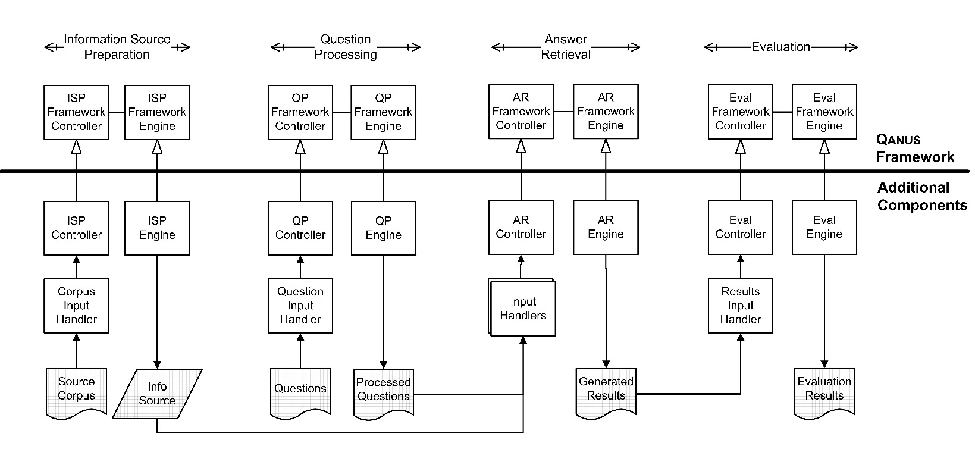
\includegraphics{graficos/Quanus}
  \caption{El framework Quanus y la implementación QA-sys}
  \label{fig:Quanus}
\end{figure}


La arquitectura, al igual que la de DeepQA, es la de un pipeline. Este
sistema consta de tres pasos principales, que se ejecutan todos por
separado (off-line): 


\bigskip

\subsection{Preparación de la fuente de información}
Este paso est\'a pensado para preprocesar cualquier base de conocimiento
y dejarla preparada para el paso 3 (retorno de la pregunta). El
framework se propone tan amplio que no hay m\'as especificaciones al
respecto. La implementaci\'on puntual asume una base de conocimiento en
formato XML de AQUAINT\footnote{\ } y la incorpora a un \'indice de
b\'usquedas Lucene. Este paso incorpora todo el conocimiento que
estar\'a finalmente offline; accesos din\'amicos a la web, por ejemplo,
se modelan en el paso 3.


\bigskip

\subsection{Análisis de la pregunta}
Este paso, igualmente gen\'erico, permite la incorporaci\'on de
distintos componentes para anotar los tokens de la pregunta con datos
\'utiles para ser consumidos por el paso 3. Otro procesamiento a
realizar en este paso podr\'ia ser la generaci\'on de queries
entendibles por los distintos motores de almacenamientos de
informaci\'on del paso 1. En particular, la implementaci\'on trae un
pos-tagger, un ner-tagger y un question classiffier, todos de Stanford.
Hablaremos m\'as de estos componentes m\'as adelante. 


\bigskip

\subsection{Generación de respuestas}
En este paso se utiliza la informaci\'on generada en la preparaci\'on
de la base de informaci\'on y en el procesamiento de la pregunta para
generar una respuesta. Tambi\'en puede incorporarse accesos a la web y
validaciones de las respuestas candidatas. La implementaci\'on concreta
eval\'ua cada pasaje de los primeros n documentos retornados por Lucene
para la pregunta original con una serie de componentes ad-hoc de
distancia para adjudicar diferentes grados de confiabilidad a los
distintos pasajes. \newline


Adem\'as, se provee de un cuarto paso opcional (el sistema de QA est\'a
completo con los tres pasos anteriores), para la fase de desarrollo y
de evaluaci\'on de la performance del sistema:\newline


\subsection{Evaluación}

Este paso est\'a pensado para evaluar las respuestas generadas y
presentarlas de un modo conciso en la fase de desarrollo.
B\'asicamente, cruza las respuestas obtenidas contra unas respuestas
esperadas escritas a mano y presenta el total de respuestas dadas
correctamente.


\bigskip

\subsection{Implementaci\'on}

El c\'odigo est\'a escrito en java y mantiene una interfaz com\'un a
todos los pasos: un controller cuyas responsabilidades son cargar los
componentes y un engine que utiliza los componentes para leer el input,
procesarlo y grabar el resultado. La adaptabilidad del framework est\'a
dada en la posibilidad de incorporar componentes respetando la interfaz
especificada para los mismos o bien, en modificar esta misma interfaz.
Presuntamente, el framework es lo suficientemente abierto para permitir
la implementaci\'on de sistemas basados en distintas fuentes de
conocimiento (ontolog\'ias, archivos, web) y con distintos modos de
funcionamiento mediante poco esfuerzo de customizaci\'on.

La implementaci\'on llamada QA-sys est\'a desarrollada para correr sobre
el tipo de datos de las evaluaciones TREC 2007 (XML AQUAINT). En el
primer paso, incorpora los XML en este formato a un \'indice Lucene, en
el segundo paso utiliza anota la pregunta con POS tags, NERs y
clasifica el tipo de respuesta con un clasificador entrenado y luego,
en el tercer paso se busca la pregunta sobre el \'indice lucene y se
retorna una lista con n documentos rankeados. Estos documentos se
subdividen en pasajes. Luego se aplican diferente algoritmos ad-hoc
dependiendo del tipo de respuesta esperada. \ Por ejemplo, si la
respuesta es un nombre de persona, se ejecuta NER sobre los diferentes
pasajes buscando nombres candidatos, si el tipo esperado es una fecha,
se utilizan expresiones regulares escritas a mano, etc. Finalmente, los
pasajes candidatos se eval\'uan utilizando heur\'isticas de proximidad
de los candidatos a la pregunta inicial. Para esto se utilizan
diferentes Scorers que rankean los pasajes seg\'un diferentes
caracter\'isticas (features) y luego se selecciona alguna priorizando
algunas caracter\'isticas sobre otras, dependiendo tambi\'en del tipo
de respuesta esperada. Por \'ultimo, el evaluador de resultados mide la
exactitud (\textit{accuracy}): total de respuestas correctas sobre
total de preguntas. QA-sys funciona s\'olo sobre preguntas del tipo
factoid y, a modo de comparaci\'on, el mejor sistema seg\'un la TREC
2007, el LymbaPA07 obtuvo un grado de exactitud del 0.706 y el d\'ecimo
(Quanta) obtuvo 0.206, mientras que QA-sys logra el 0.119. La
implementaci\'on es realmente simple y funciona s\'olo a modo de
ilustraci\'on de lo que puede construirse sobre el framework. 

\bigskip

\section{Otros sistemas de QA: OpenEphyra, Aranea y Just.Ask}

\bigskip

El paper describe las arquitecturas de todos los sistemas, si sirve
meter m\'as info

El paper [EPHYRA1] \ busca crear un criterio cuantitativo para comparar
la eficacia de distintos pasos de Just.Ask, Open Ephyra y Aranea
bas\'andose en la arquitectura \textit{pipeline de tres pasos}
compartida por todos. Los tres sistemas, por lo dem\'as, est\'an
basados en la web, utilizando distintas APIs de buscadores o bien
analizando los resultados de la interfaz de usuario de los mismos. 

El primer \'item importante a destacar de este trabajo, es que, al
momento de la experimentaci\'on \textbf{Aranea no funcionaba m\'as y
estaba discontinuado}\footnote{\ (Resaltado en Secci\'on 8, muy
concluyente).\par }\textbf{. }El autor se comunic\'o con el responsable
del proyecto que corrobor\'o que las APIs de los buscadores en los que
se basaba Aranea cambiaron y no hab\'ia inter\'es en readaptar el
c\'odigo para que vuelva a funcionar. Las comparaciones que logr\'o
entre Just.Ask y Open Ephyra son interesantes y concluyentes a favor de
la performance de OpenEphyra. 

(Freeling \ + Cambio de Base + Rigidez)

\chapter{Implementación}

\section{Frameworks}

\subsection{No funcionales}

Para la implementación de nuestro sistema, originalmente, evaluamos la
utilización de distintos frameworks disponibles. DeepQA, el producto
de IBM, no es de código abierto, por lo que acerca de su
implementación sólo sabemos lo que ventilaron en sus artículos
técnicos. Just.ask, el sistema basado en web comparado contra
OpenEphyra no está disponible en la web al momento de escribir este
trabajo, mientras que OpenEphyra no funciona tal cual está dise\~nado
originalmente (basado en web), sino que el autor sugiere unos pasos
esotéricos para configurarlo para usar conocimiento local. Cabe
destacar que esta falla en la funcionalidad está asociada a la que
había encontrado [AUTOR DE PAPER EPHYRA1] en Aranea y está
vinculado con una serie de medidas restrictivas tomadas por las
compa\~nías de buscadores, que fueron cerrando sus accesos gratuitos
para la comunidad de investigación bloqueando sus APIs y el acceso
automático a sus UI. Las alternativas para el uso de buscadores,
actualmente, se reducen a la configuración de una serie de proxies
sobre los que rotar el acceso a la UI y así enga\~nar al detector de
accesos automáticos -alternativa de legalidad cuestionable - o bien al 
pago por una quota de queries por mes.
OpenEphyra sobrevivió a Aranea porque sus responsables escribieron
una interfaz para Bing cuando Google cerró sus puertas, mientras que
los responsables de Aranea no lo hicieron. Finalmente, Bing también
bloqueo el acceso automático gratuito. Notar que el mismo tipo de
discontinuación ocurrió con el API de traducciones de Google. La
empresa declara, explícitamente, que no está dispuesta a acceder a
ninguna quota de acceso gratuito para la investigación académica y
que todos sus servicios son pagos. 

%Tanto de Aranea como de OpenEphyra podríamos llegar a tomar algunos de
%sus componentes a la hora de construir nuestro sistema. Por el momento,
%fueron simplemente dejados de lado.

\bigskip

\subsection{Qanus}

Finalmente, un sistema que \textit{sí} estaba disponible y funcionando
fue Qanus, que respetaba al pie de la letra su detalle técnico. Al comienzo
del proyecto, contábamos con un corpus de datos en XML,
lo cual coincidía, al menos en gran parte, con el input esperado de
la implementación Qa-sys. A pesar de esto, la adaptación de los
componentes no fue nada trivial y requirió un tiempo excesivo. En
particular, existían dos opciones a la hora de construir un sistema
sobre la arquitectura Qanus: dejar de lado la implementación Qa-sys e
implementar todos los componentes de cero sobre la arquitectura, respetando las interfaces
dadas por el framework, o adaptar el sistema funcionando para que
trabaje sobre los nuevos datos y el nuevo entorno esperado. Frente a
esta alternativa, se aparece claro que el framework en sí mismo no
aporta demasiado, pues lo único que hace es atar la implementación
final a una interfaz estructurada de tres procesos bastante sencillo.
Además, existe un cierto grado de dependencia de la arquitectura
hacia la implementación final, quizás no a nivel técnico, pero si
en el modo en el que está definida la estructura. Por este motivo,
encaramos una adaptación de Qa-sys a nuestro modelo de datos y a
nuestros requerimientos, pero los resultados no fueron buenos en
términos de resultados por tiempo invertido. El tiempo de aprendizaje
del framework mismo y el tiempo requerido para adaptar las distintas
componentes propias a las interfaces esperadas por Qanus es demasiado
alto para la solución que brinda. Como recién mencionamos, en
realidad, el proceso de pipeline de tres pasos no tiene tantas aristas,
y adaptarse a un framework es mucho menos ameno que escribirlo. Este
puede ser uno de los motivos por los cuales, como acertadamente
se\~nalan los autores de Qanus, no existe ningún framework
estandarizado dentro del ámbito de la investigación en QA.
Después de la investigación inicial, podríamos concluir que
está estandarizado, al menos a modo conceptual, la idea de que la
resolución del problema se debe enfocar como un pipeline de al menos
tres pasos que incluyen:
\begin{itemize}
\item el preprocesamiento de la base de conocimiento,
\item el preprocesamiento de la pregunta,
\item el retorno de la respuesta a partir de los resultados de los dos pasos anteriores. 
\end{itemize}
Como último comentario al respecto, el modelo de Qanus resultaba poco atractivo
 a la hora de incorporar procesamiento en varios idiomas: el mejor approach
utilizando esta arquitectura era implementar dos sistemas basados en
Qanus paralelos y utilizar uno u otro de acuerdo con el resultado de
una detección inicial. 

\bigskip

Si bien el modelo de Qanus fue, por los motivos recién expuestos,
dejado de lado, debemos destacar una serie de puntos en los que fue
útil.

En primer lugar, uno de los objetivos de Qanus es facilitar el ingreso
al área del QA de nuevos investigadores. Creemos que esto está
logrado perfectamente: el código es muy sencillo y claro y lo mismo
ocurre con la documentación, lo que hace de Qanus un proyecto muy
útil desde una perspectiva pedagógica o educativa, más allá de
que sea esta misma simpleza la que más adelante atente contra la
usabilidad. El modelo de pipeline, que es el enfoque teórico usual al
problema, y los distintos componentes y usos típicos de estos
componentes en los distintos pasos del pipeline se realizan linealmente
en la implementación de Qanus y Qa-sys. En particular, la similaridad
entre la descripción del código de IBM (DeepQA y Watson) y el
enfoque con el que Qanus ataca el mismo problema salta a la vista,
considerando la diferencia de escalas. 

En segundo lugar, en el plano de la investigación del estado de arte
de los sistemas de QA disponibles creemos que el intento con Qanus
redundó en un cierto escepticismo sobre la posibilidad de resolver
nuestro problema utilizando herramientas disponibles de gran escala. La
conclusión es análoga a la que tuvo el equipo de IBM al intentar
usar OpenEphyra y PIQUANT: el tiempo de customización y adaptación
de los framework a nuestro problema puntual es demasiado alto en
comparación con el tiempo necesario para construir una nueva
arquitectura que cumpla los mismos requisitos. 

Por último, en un nivel técnico, Qanus nos resultó de utilidad para
construir nuestro modelo final pues reutilizamos varios de los
componentes de Qa-sys: En primer lugar, recuperamos el POS tagger, el
NER tagger y el Question Classiffier (QC) de Stanford, que son las
librerías principales con las que Qa-sys encara el procesamiento
lingüístico de la pregunta y parte del proceso de generación de
respuestas. Todas estas herramientas están disponibles en la web por
otros medios, pero algunas -principalmente el QC- requieren un cierto
tiempo de configuración inicial que los autores de Qanus ya habían
resuelto. Es decir, reutilizamos, además de estos módulos externos,
bastante de la configuración y las APIs de acceso a estos módulos
escritos por los singapurenses. Estas herramientas funcionan bien
sólo para inputs en inglés. Las adaptaciones que hicimos las
veremos más abajo. Por otro lado, incorporamos casi sin
modificaciones algunas métricas de distancia entre pasajes que Qa-sys
usa en el momento de la generación de la respuesta como Scorers.
Estos son las clases: \textbf{FeatureSearchTermCoverage},
\textbf{FeatureSearchTermFrequency}, \textbf{FeatureSearchTermProximity},
\textbf{FeatureSearchTermSpan}. Explicaremos esta métricas en breve, dentro de nuestro
modelo, bajo en nombre de
{\textquotedblleft}Comparadores{\textquotedblright}. Este código
está escrito por los autores de Qanus (es decir, no es una librería externa utilizada por ellos).


\bigskip

\section{Arquitectura}

\subsection{Motivación}

Después del intento con Qanus, decidimos implementar el sistema por
fuera de cualquier framework y encaramos el dise\~no actual. En este
dise\~no respetamos el modelo típico de pipeline de tres pasos que
abunda en la literatura científica y, por lo demás, parece el
indicado a la hora de encarar este tipo de problemas. Un momento no-técnico
importante a destacar es la obtención de una base de datos en
mongodb, resultado del trabajo del proyecto MITIC, la cual cambió
sustancialmente el enfoque anterior, basado en XMLs. 
A partir de estos datos, fue posible delinear un esquema de entidades formal que determinó
qué se puede responder y qué no. Como vimos, la estrategia de QA
cuando el tipo de datos es estructurado es radicamente distinta que la
estrategia cuando los datos son no estructurados. Qanus, por su parte,
está orientado a un tipo de datos no estructurados: buscar documentos
rankeados en un índice de búsqueda y rastrear en ellos pasajes
mediante distintos métodos. Cuando la base de conocimientos consta de
un tipo de datos estructurado (esto es, de entidades, relaciones,
atributos de entidades) es posible delimitar una ontología más
rígida que permita concentrarse en la interpretación de la pregunta
hacia un lenguaje formal. El arquetipo de este enfoque puede pensarse
como la traducción de un lenguaje de consulta humano a un lenguaje de
consulta formal, como por ejemplo, SQL: esta estrategia de QA puede
entenderse \ como una interfaz inteligente a una base de datos. \ En
eje principal en este acercamiento está en el análisis
lingüístico de la pregunta a fin de mapearla a un dominio conocido
y, por otro lado, no es necesario hacer análisis lingüístico
sobre el corpus de datos.

Por otro lado, dado que nuestro objetivo inicial incluía desarrollar
métodos de QA con soporte bilingüe basados en textos (datos no estructurados) 
y esta base de conocimiento no lo permite, incorporamos al proyecto la resolución
algunos de los ejercicios de la competencia QA4MRE (Question Answering for Machine Reading Evaluation)
de la CLEF (Cross-Language Evaluation Forum) del a\~no 2007. 

Estos ejercicios fueron elegidos para poder evaluar nuestros métodos de análisis lingüsticos,
ya que la naturaleza del dominio de conocimiento del proyecto mitic - por el formato de sus datos
 y por lo puntual de su temática- hace imposible cualquier métrica de evaluación objetiva.
Tras investigar distintas competencias y métodos de evaluación, optamos por la CLEF del 2007
por contar con un subconjunto de ejercicios bastante adecuados para nuestro sistema mientras que el corpus
de datos necesario para completar estos ejercicios estaba (en parte) disponible dentro de los tiempos 
requeridos por nuestro proyecto. 

\bigskip

\subsection{Modelo}

Nuestro sistema resuelve dos problemas de QA similares pero distintos. 

Por un lado, disponemos de una base de datos estructurada, con datos del área de la investigación y la
producción en TICs en Argentina, que requiere un enfoque estructurado con métodos basados en ontologías y en 
formalizaciones de dominio. El enfoque aquí es traducir la pregunta formulada en lenguaje humano a un lenguaje más
formal ``comprensible" según el modelo de dominio. 

Por otro lado, para evaluar métodos de QA 
para datos no estructurados, resolvimos algunos ejercicios de la competencia CLEF del '07. La base de conocimientos para
estos ejercicios son algunos snapshots de Wikipedia en Espa\~nol y en Inglés, anteriores al 2007. Sobre esta base de conocimiento,
el enfoque no es ``traducir" la pregunta a un lenguaje estructurado sino interpretarla y ``compararla", mediante distintas métricas, 
con documentos y pasajes, buscando medidas estádisticas y otras condiciones que permitan \textit{rankear} una respuesta candidata
con un cierto grado de confianza, o bien determinar que no fue posible encontrar una respuesta para la pregunta. 


Conceptualmente, el modelo consiste en los tres pasos típicos: la
creación de la base de conocimientos optimizada, el análisis
lingüístico de la pregunta y la generación de una respuesta desde
la base de conocimientos optimizada a partir de la pregunta con sus
anotaciones. 
Los pasos 1 y 2, la generación de la base de conocimientos optimizada y el procesamiento de la pregunta son procesos
esencialmente análogos para la base de conocimientos estructurada y para la no estructurada. El tercer paso, la generación de respuestas,
tiene distintos enfoques según el caso. 
En las siguientes secciones recorreremos ambos enfoques en conjunto, señalando las decisiones de dise\~no y los distintos módulos
utilizados, haciendo las distinciones pertinentes cuando sea necesario.

En las secciones subsiguiente comentaremos las implementaciones de los
distintos pasos, con sus decisiones de dise\~no y las tecnologías
utilizadas. 


\bigskip

\section{Base de conocimiento}
\bigskip


La creación de la base de conocimiento es el único que se ejecuta offline
y consiste en la obtención del corpus original y en la generación de índices
invertidos. Los índices invertidos, recordamos, son índices que permiten
buscar, para una serie de términos vinculados lógicamente, un conjunto
ponderado de documentos pertinentes. Por su naturaleza, este paso está 
separado de la ejecución del resto del código.

\subsection{Corpus inicial}

\subsubsection{Grafo Mitic}
Los datos originales del proyecto mitic constan de una serie de documentos 
xml y de cinco colecciones de mongodb y relaciones entre ellas (una base de datos no relacional).

Las cinco coleccciones son: universidades, investigadores, empresas,
publicaciones, proyectos y temáticas.

Estas colecciones definen el dominio. Cada entidad 
posee sus respectivos atributos y distintas relaciones con otras entidades.
Estas relaciones contienen desde vínculos explicitos como "trabajar-en"
pero también relaciones inferidas mediante distintos algoritmos durante el proyecto mitic.
Las relaciones que incorporamos tienen distintos pesos según este tipo de caracteristicas
y tejen un grafo de distancias más o menos "especulativas" entre todas las entidades.

Los atributos de cada entidad se pueden ver en el Anexo: [[HACER Y LINKEAR]].

\subsubsection{Wikipedia}
El subset de ejercicios de CLEF'07 que elegimos resolver
utiliza como corpus un snapshot de wikipedia en inglés y otro en español,
ambos anteriores al año 2007.
El set de preguntas completo involucra una serie de documentos para los cuales hay que 
registrarse en la asociación: algunas preguntas se responden en base a wikipedia y otras en base a estos documentos.
Identificamos las preguntas que se responden desde wikpedia chequeando los documentos fuente de las respuestas esperadas.

Wikipedia ofrece diferentes formas para obtener una propia imagen de la enciclopedia.
Es posible incorporar la base de datos de wikipedia a una instalación wikimedia
propia, es posible descargar una imagen estática del sitio en archivos html y también se puede
descargar un archivo xml gigante con todos los artículos. 

En la guía para los participantes de la competencia \cite{Clef07} hay un link para descargar 
wikipedia en inglés preprocesada de Noviembre de 2006 \footnote{\url{http://ilps.science.uva.nl/WikiXML/}} y dos opciones para descargar wikipedia en español: una imagen estática en html de Noviembre de 2006 \footnote{\url{http://static.wikipedia.org/downloads/November_2006/es/}} y un dump xml de Diciembre de 2006 
\footnote{\url{http://download.wikimedia.org/images/archive/eswiki/20061202/pages-articles.xml.bz2}}

La guía aclara que, bajo responsabilidad de los participantes, se puede usar
cualquier otra versión de Wikipedia, siempre y cuando sea anterior a noviembre / diciembre de 2006.
Además, se pide que las respuestas sean tomadas de ``entradas reales" o artículos de wikipedia y
no de otros documentos (por ejemplo: ``image", ``discussion", ``category", etc).

Los links a páginas de wikipedia en español no estaban más disponibles (ambos respondieron 404), mientras que el formato
preprocesado pedido para el inglés resultaba realmente complejo de instalar y parecía una linea muerta. Por estos motivos,
seguimos la sugerencia sobre el uso responsable de otras wikipedias y utilizamos las siguientes:

\medskip

\begin{center}
\begin{tabular}{ | l | l | l |}
    \hline
    Idioma & Fecha & Tamaño\\ \hline
    Inglés \footnote{\url{http://dump-ingles-1}} & 4 de noviembre de 2006 & 7,6G \\ \hline
    Español \footnote{\url{http://dump-español-1}} & 7 de julio de 2006 & 558M \\ \hline
\end{tabular}  
\end{center}

El mantenimiento de un mismo formato para ambos idiomas nos permitió crear un indexador único para cualquier
dump en xml de una wikipedia. Durante el desarrollo y las pruebas, para evitar tiempos de carga innecesarios y también
para probar, utilizamos otras imagenes disponibles de wikipedia:

\medskip

\begin{center}
\begin{tabular}{ | l | l | l |}
    \hline
    Idioma & Fecha & Tamaño\\ \hline
    Español & 26 de enero de 2007 & 902M \\ \hline
    Español & 14 de junio de 2013 & 7,3G \\ \hline
    Inglés simple & 4 de julio de 2006 & 26M \\ \hline
    Inglés simple & 24 de julio de 2013 & 406M \\ \hline
 \end{tabular}
\end{center}


\subsection{Creación de Indices}

\begin{figure}[H]
  \centering
    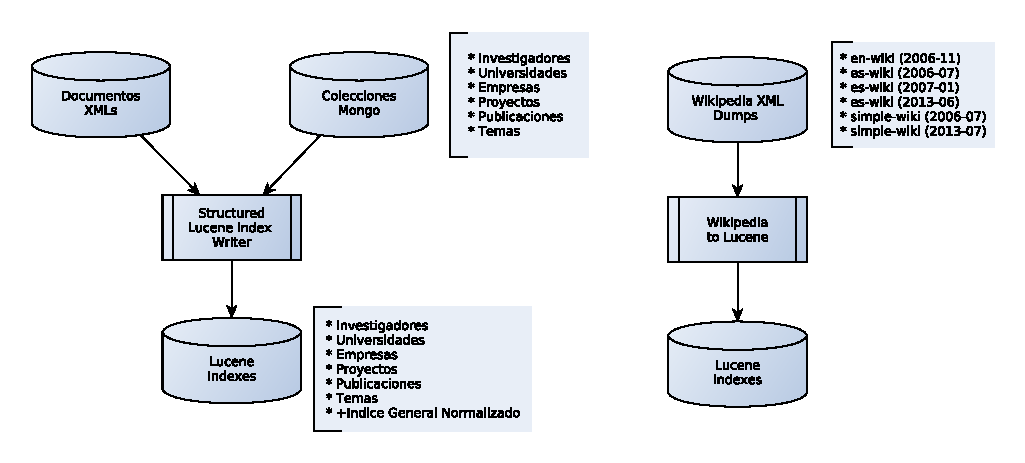
\includegraphics[scale=0.86]{graficos/LuceneWritersJuntos}
  \caption{Creación de Indices}
  \label{fig:LuceneIndexWriterBoth}
\end{figure}

A partir de esta base de datos de mongo y de los archivos xml fueron construidos cinco índices
de búsqueda lucene y un índice de búsqueda más, general, con la
información normalizada de los otros cinco. 
Cada uno de los cinco índices por entidad mantiene la estructura del tipo como campos de los documentos.
Esto quiere decir que el índice invertido para \emph{Investigadores} tiene los mismos campos
del modelo de datos de nosql. Además, se agregó el campo ``all" que resulta de la concatenación de
todos los campos. Este campo resulta útil a la hora de filtrar resultados. 
El índice general posee un documento por cada entidad de las cinco colecciones, 
manteniendo también un puntero a la entidad original y su tipo.
%El proceso de creación de índices se ilustra en la Figura \ref{fig:LuceneIndexWriterEstructurado}%~\nameref{fig:LuceneIndexWriterEstructurado}.

% \begin{figure}[H]
%   \centering
%     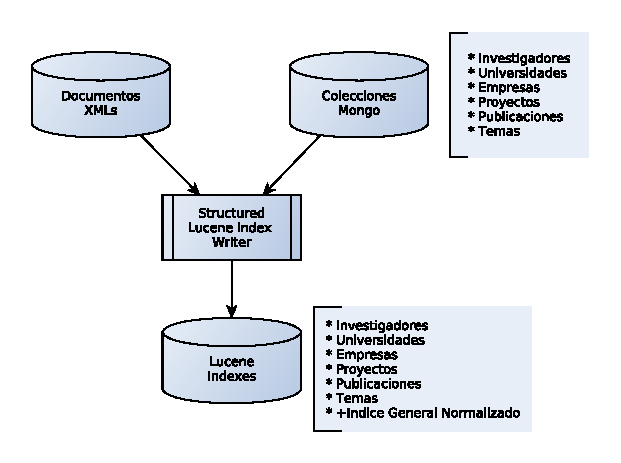
\includegraphics{graficos/LuceneIndexWriterEstructurado}
%   \caption{Lucene Index Writer para datos del proyecto Mitic}
%   \label{fig:LuceneIndexWriterEstructurado}
% \end{figure}

Para la construcción de indices lucene con los dumps de wikipedia usamos la librería gwtwiki (Ver Apéndice~\ref{sec:gwtwiki}).
Los artículos se indexan como documentos con los siguiente campos: \emph{id, title, body y all}. En este proceso se descartan artículos mal formados y 
entradas representado imágenes o discusiones, tal como se sugiere en la guía. 
Por mera curiosidad, tomamos tiempos en la contrucción de estos índices locales sobre versiones de wikipedia.
Estos son algunos tiempos de indexación para distintos dumps sobre una [[detalles de la compu]]:
\begin{center}
\begin{tabular}{| l | l | l | l |}
\hline
Idioma & Tamaño & \# Entradas & Tiempo \\ \hline
es & 50M & \# 16 millones & 2.5min \\ \hline
es & 50M & \# 16 millones & 2.5min \\ \hline
es & 50M & \# 16 millones & 2.5min \\ \hline
es & 50M & \# 16 millones & 2.5min \\ \hline
\end{tabular}
\end{center}

El proceso de creación de índices está ilustrado en la figura \ref{fig:LuceneIndexWriterBoth}



% \begin{figure}[H]
%   \centering
%     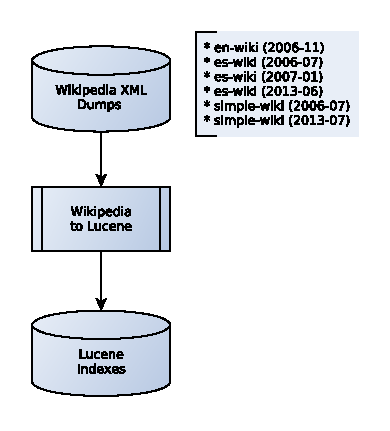
\includegraphics{graficos/LuceneIndexWriterWiki}
%   \caption{Lucene Index Writer para dumps de Wikipedia}
%   \label{fig:LuceneIndexWriterWiki}
% \end{figure}



\subsection{Interfaz de servicios}
\label{subsec:modelos-db}
La creación offline de índices lucene tiene como finalidad optimizar
la base de conocimiento para responder con mayor eficiencia 
a búsquedas de resultados en un momento posterior. 

En esta sección vamos a ver la interfaz que presenta la base de conocimientos indexada 
al resto de los módulos del sistema y qué dependencias existen con los módulos de
análisis lingüístico.

Para la base de conocimiento estructurada, reutilizamos un modelo de datos
escrito en java  del grafo de entidades que obtuvimos de los investigadores del proyecto mitic (Ver \allref{sec:modelos-morphia}).
A estos modelos se les agregó soporte para su representación como documento dentro de un índice.
Por ejemplo, el modelo para la entidad ``Universidad de Buenos Aires", además de
persistirse en la colección de universidades de la base de datos de mongo, también dispone de una representación como documento en 
un índice lucene particular (el índice de universidades) y otra en el índice general.
A nivel colecciones, cada entidad dispone de un representante que maneja el acceso a su colección en la base de datos y también a su índice. A partir de estos representantes por entidad que ofrecen acceso a una base de datos y a un índice creamos la interfaz \emph{KnowlegdeBase}. 
Cada entidad tiene una interfaz de administración de sus dos motores de persistencia. Las responsabilidades de esta interfaz son las de un handler de conocimiento acerca de una cierta clase de entidades. 
Además, esta interfaz permite la reificación de entidades implicitas en el modelo. Estas entidades son: Ciudad, Provincia, Centro de Investigación, etc \footnote{hacer y escribir bien}. Esta reificación significa abstraer las funciones directas contra la base de datos. Mientras el $KnowledgeBase$ de Investigadores habla directo contra la base mongo o contra lucene, el $KnowlegdeBase$ de Ciudades habla contra Investigadores, Universidades y Empresas verificando ciertos campos y recomponiendo la forma de la entidad, de modo abstracto y sin persistencia propia. 

[[Tablita con totales por entidad]]

\bigskip

[[Relaciones solo presentes en mongo]]

\bigskip

Las $KnowledgeBase$ de las cinco entidad y el índice general están, a su vez, controlados un $KnowlegdeManager$, que es la interfaz del módulo que maneja la base de conocimiento. 

El $KnowledgeManager$ ofrece diferentes servicios de verificación de entidades. Para una cadena de tokens cualquiera, este módulo puede decidir, con un cierto grado de confianza, los siguientes problemas:

\begin{itemize}
  \item Si la cadena de tokens es una entidad dentro del modelo de datos. Esto incluye:
    \begin{itemize}
      \item Es una entidad del modelo de datos: una universidad, una empresa, un investigador, un proyecto, una publicacion o una tematica
      \item Es una entidad inferida: una ciudad, una provincia, un centro de investigación, un lugar de trabajo
    \end{itemize}
  \item Si la cadena es una colección del modelo de datos, es decir, si se están nombrando \dblquote{Investigadores} o \dblquote{Universidades} como clase de entidades.
  \item Si la cadena es un atributo o una relación de una clase de entidades.
\end{itemize}

La primer verificación utiliza campos de identidad de las entidades y diferentes tipos de comparadores (Ver apéndice \allref{sec:comparadores} ). Cada entidad fue configurada con diferentes atributos de identidad y a su vez estos atributos están asociados a diferentes comparadores a con un cierto grado de peso y de confianza en el juicio general. 

La segunda y la tercera verificación utiliza estos mismos comparadores jerarquizados, pero compara las cadenas de entrada contra diccionario de sinónimos escrito a mano nombrando las diferentes clases de entidades y los atributos de cada una de ellas. 

\begin{figure}[H]
  \centering
    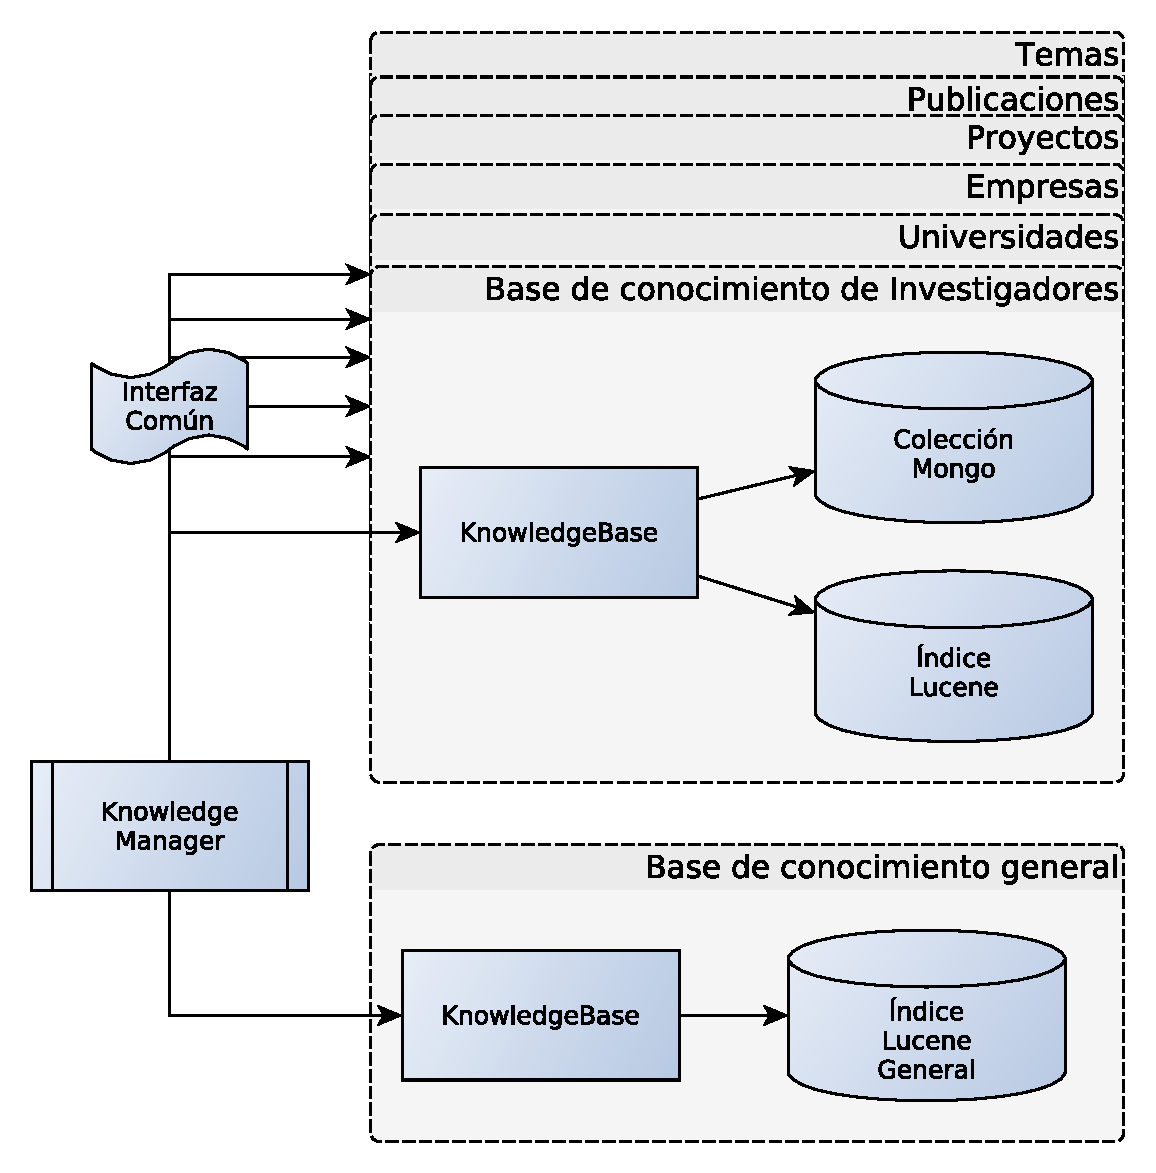
\includegraphics[scale=0.5]{graficos/KnowledgeManager}
  \caption{Base de Conocimiento de grafo de TICs}
  \label{fig:KnowledgeManager}
\end{figure}

\bigskip

La base de conocimiento de los ejercicios de Clef '07 es mucho más sencilla 
porque no existe ningún modelo \emph{a priori} más allá del documento de lucene.
El formato de la entidad ``artículo", como señalamos antes, es: $(id, titulo, cuerpo)$. 
En este caso, el trabajo más fino no está en el modelado inicial del dominio 
sino la capacidad lingüística de extraer pasajes a partir de un artículo y recomponer información
estructurada a partir de estos pasajes. Mientras que para un modelo estructurado la base de conocimiento
debería permitirnos, para un cierto input, identificar univocamente una entidad y darnos pistas sobre un pedido de
información acerca de esa entidad, el objetivo sobre un corpus de documentos en 
traer todos los documentos en los que sea posible que exista un pasaje respondiendo a la pregunta o
evidencia relevante para apoyar una respuesta. Es decir, mientras una respuesta acotada es una virtud para
el manejador de una base de conocimientos estructurada, el manejador de una lista de documentos de texto debería devolver
una lista lo suficientemente grande para contener la respuesta dentro de los pasajes. La razón de esta política es que si
por ser demasiado estrictos a la hora de retornar documentos llegasemos a descartar un pasaje candidato válido esto
redundaría en una baja generar de efectividad, mientras que en pasos subsiguiente será trivial descartar toda información irrelevante
sin tanto costo. Por eso, el acceso a los indices de wikpedia consta simplemente de un generador de queries similar al recién comentado
accediendo y acumulando resultados (rankeados) a partir de un $LuceneIndexReader$ común (Ver \ref{sec:lucene} \nameref{sec:lucene} para más información).


\bigskip

\section{Análisis de la pregunta}
\label{sec:qprocess}
En este paso se realizan diferentes análisis lingüísticos de la pregunta.
El resultado son distintas características asociadas a la pregunta (anotaciones)
y distintas entidades semánticas reconocidas útiles para el proceso de generación de respuestas. 
Las herramientas de procesamiento de lenguaje natural que utilizamos en 
la implementación de este paso del pipeline 
incluyen: detección de lenguaje, extracción y verificación de entidades nombradas (NER), 
de verbos, sustantivos, qwords (qué, quién, cómo) (POS), análisis de n-gramas y categorización por tipo de pregunta (QC).

El proceso de análisis de la pregunta es bastante similar para ambos approachs (estructurado y no estructurado), por lo
que comentaremos ambos en simultaneo, mencionando diferencias cuando corresponda. 
Estructuraremos esta parte de la tesis en las siguientes secciones:

\begin{itemize}
\item Detección de idioma 
\item Detección y verificación de entidades nombradas
\item Análisis gramatical
\item Clasificación del tipo de pregunta
\end{itemize}

Si bien es cierto que el segundo item está basado principalmente en NER-tagging, el tercero en POS-tagging y el cuarto en Question Clasiffication, 
cada uno de estos pasos utiliza estas herramientas de diferentes maneras. Por ejemplo, para la detección y verificación de entidades del analisis estructurado, además del NER-tagger también utilizamos la base de conocimiento y el análisis gramatical y, para el español, la clasificación del tipo de pregunta se hace apoyandose en las qwords identificadas por el POS-tagger.

\subsection{Idioma}

\begin{figure}
  \centering
    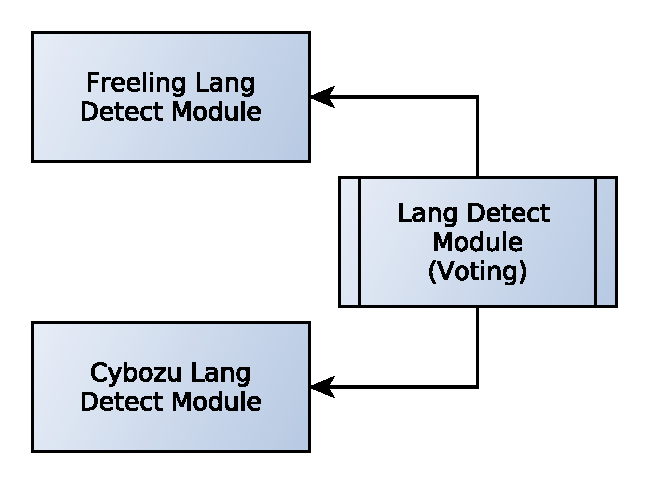
\includegraphics[scale=0.5]{graficos/LangDetect}
  \caption{Módulo de Detección de Idiomas}
  \label{fig:LangDetect}
\end{figure}

El módulo de detección de idiomas de nuestro sistema utiliza dos librerías distintas.
El módulo de detección de idiomas de Freeling y una librería especializada de Cybozu Labs. (Ver apéndices \allref{sec:freeling} y \allref{sec:cybozu} para más información)

Ambos permiten priorizar la detección de ciertos idiomas sobre otros desde su configuración.
De esta manera podemos forzarlos a identificar sólo los idiomas esperados en nuestro dominio. 
Ambos fueron configurados para detectar inglés y español para mejorar la confiabilidad,
pero pueden habilitarse más idiomas de ser necesario y funcionan correctamente. 

El módulo de detección simplemente evalua ambos algoritmos y 
decide el resultado con un cierto grado de confianza. En caso de existir un empate, se 
prioriza la opción de Cybozu labs que en la práctica dió resultados más exactos.

De todos modos, el problema "detección de idioma" no introduce mayores complicaciones y parece un problema bien resulto.
Es decir, la mayoría de las veces ambos módulos responden lo mismo y de modo correcto.
Sin embargo, para ciertos casos bordes molestos (pero lamentablemente frecuentes)
el detector de Cybozu resultó funcionar mejor. Por ejemplo, está el caso de la pregunta formulada en inglés pero acerca de una entidad nombrada en español: 
``Where is located the Universidad de Buenos Aires?". Este problema está particularmente presente en el procesamiento de preguntas -nuestra tarea-, dado que son textos cortos en los que una construcción sustantivada en otro idioma puede desequilibrar erróneamente la balanza. 

A continuación presentamos algunos ejemplos que ilustran el funcionamiento de ambas librerías y el resultado final de nuestro módulo en estos casos:

\begin{center}
\begin{tabular}{| p {8cm} | l | l | l |}
\hline
Texto & Freeling & Cybozu & Resultado \\ \hline
¿Dónde queda la Universidad de Buenos Aires? & es & es & es \\ \hline
Where is located the University of Buenos Aires? & en & en & en \\ \hline
Where is located the Univesidad de Buenos Aires? & en & en & en \\ \hline
Where is located Universidad de Buenos Aires? &  {\color{red}es} & en & en \\ \hline
Quién es Carolina Fernandez? & es & es & es \\ \hline
Who is Carolina Fernandez? &  {\color{red}none} & en & en \\ \hline
Quién es John McCain? & {\color{red}none} & es & es \\ \hline
Who is John McCain? & en & en & en \\ \hline
Dónde vive John McCain y por qué vive allí? & es & es & es \\ \hline
Where does Carolina Fernandez live and why does she lives there? & en & en & en \\ \hline
\end{tabular}
\end{center}

Los ejercicios de Clef '07 no evaluan detección de idiomas. Los archivos de preguntas están separadas por idioma y no se espera que el idioma se infiera a partir de los textos de las preguntas, sino que es un dato dado al sistema de QA.

\subsection{Entidades nombradas}
\label{subsec:impl-ner}

Para la detección de entidades utilizamos la clase simple de detección (NER) y clasificación (NEC) de entidades de Freeling y el NERC de Stanford (ver \allref{sec:freeling} y \allref{sec:stanford-ner}). Las herramientas de Stanford en general superan a las de Freeling -al igual que el detector de idiomas de Cybozu-, pero solo sirven para inglés. La clasificación utilizada por ambos es la más general de las comentadas en \allref{subsec:nerc}: persona, lugar, organización y otros. 

Veamos algunos ejemplos de funcionamiento de los módulos de detección de entidades. 

\begin{center}
\begin{tabular}{| p {8cm} | l | l | l |}
\hline
Texto & Freeling & Stanford & Resultado \\ \hline
¿Dónde queda la Universidad de Buenos Aires? & es & es & es \\ \hline
Where is located the University of Buenos Aires? & en & en & en \\ \hline
Where is located the Univesidad de Buenos Aires? & en & en & en \\ \hline
Where is located Universidad de Buenos Aires? &  {\color{red}es} & en & en \\ \hline
Quién es Carolina Fernandez? & es & es & es \\ \hline
Who is Carolina Fernandez? &  {\color{red}none} & en & en \\ \hline
Quién es John McCain? & {\color{red}none} & es & es \\ \hline
Who is John McCain? & en & en & en \\ \hline
Dónde vive John McCain y por qué vive allí? & es & es & es \\ \hline
Where does Carolina Fernandez live and why does she lives there? & en & en & en \\ \hline
\end{tabular}
\end{center}

\medskip

Mientras la detección de entidades para los ejercicios de Clef se detiene en el reconocimiento de entidades nombradas a nivel lingüísitico, para el sistema estructurado el proceso es un poco más complejo. Esto se debe a que en este caso la detección de entidades es esencial. Si en el proceso de anotado de la pregunta no se logra identificar alguna entidad reconocida por el modelo de datos, entonces se está muy lejos de encontrar una respuesta. Por eso, además de utilizar los modulos NER recién mencionado, agregamos otros algoritmos de detección y, también, verificación de entidades. 

En principio, verificamos la o las entidades nombradas reconocidas contra la base de conocimiento. El $KnowledgeManager$ ofrece diferentes servicios de verificación de entidades. Para una cadena de tokens cualquiera, este módulo puede decidir, con un cierto grado de confianza, si:

\begin{itemize}
  \item La cadena de tokens es una entidad dentro del modelo de datos. Esto incluye:
    \begin{itemize}
      \item Es una entidad del modelo de datos: una universidad, una empresa, un investigador, un proyecto, una publicacion o una tematica
      \item Es una entidad inferida: una ciudad, una provincia, un centro de investigación, un lugar de trabajo
    \end{itemize}
  \item La cadena es una colección del modelo de datos, es decir, si se están nombrando \dblquote{Investigadores} o \dblquote{Universidades} como clase de entidades.
  \item La cadena es un atributo o una relación de una clase. (nombre de investigador)
\end{itemize}

Parte importante del trabajo para este esquema es lograr identificar este tipo de entidades lingüísticas, por lo que además de verificar los resultados del proceso de NER-tagging, también generamos otras cadenas de input. Notar además que los nombres de clase y de atributos de clase no tendrían por que ser reconocidas por el NER-tagger. Por ejemplo, para ``¿Qué investigadores trabajan en Córdoba?", \dblquote{investigadores} está haciendo referencia al nombre de una clase pero no es el tipo de entidades lingüísticas que detecta un NER-tagger. 

Por estas razones, generamos más entidades lingüísticas posibles además de las entidades detectadas por los NER-taggers. Una vez que todas las entidades nombradas fueron verificadas, generamos n-gramas sobre el resto de la pregunta para chequear por más tokens reconocibles. Configuramos la generación de n-gramas de 1 a 3, con ciertos filtros para no verificar construcciones que no representan entidades de manera trivial. Por ejemplo: dejamos sólo los unigramas que cumplan el rol de sustantivos, eliminamos bigramas que sean un sustantivo y una acción, salteamos NERs ya reconocidas, etre otros.


\subsection{Análisis gramatical}

De las diferentes etiquetas que generan los POS-taggers, en nuestro sistema distinguimos los verbos, los sustantivos, las qwords y las palabras triviales. 
Las palabras etiquetadas cumplen distintos roles a lo largo del proceso de generación de respuestas. Como señalamos recién, los n-gramas que se verifican contra la base de datos están filtrados por los roles gramaticales de sus tokens. Por otro lado, a la hora de generar el tipo de pregunta para una pregunta en español, utilizamos, como mecanismo ad-hoc, las qwords. 

\begin{center}
\begin{tabular}{| l | l |}
\hline
Clase & Ejemplos\\ \hline
qword  & qué, quién, cómo, dónde, cuándo\\ \hline
verbo & trabaja, trabajar, trabajando \\ \hline
trivial  & lo, a, de, y \\ \hline
sustantivos  & universidad, impresora, álgebra \\ \hline
\end{tabular}
\end{center}

Los usos más intensivos de estas etiquetas son el filtrado de n-gramas que describimos en la sección anterior para el caso estructurado (\allref{subsec:impl-ner}), un algoritmo ad-hoc de etiquetado de Q-Type para el caso español (es el próximo tema a discutir en \allref{subsec:qtype}) y, para la generación de respuestas, las ponderaciones de pasajes en los scorers de los ejercicios de Clef (\allref{subsec:scorers}), y finalmente, sirven para desempatar por atributos o relaciones preguntadas en algunos casos del modelo estructurado.

\subsection{Clasificación}
\label{subsec:qtype}
Para clasificar la pregunta según su tipo de respuesta esperada utilizamos el Question Classiffier de Stanford, tomando la configuración de Qanus. Este clasificador arroja una clase y una subclase (ver \allref{sec:stanford-qc} para una lista detallada de las posibles clases) y un grado de confianza para esta asignación. A continuación presentamos algunos ejemplos que ilustran estos resultados.

\begin{center}
\begin{tabular}{| l | l | l |}
\hline
Pregunta & Clase y Subclase & Confianza\\ \hline 
What's his name? & HUM:ind & 0.74 \\ \hline 
Where do you come from? & DESC:desc & 0.62 \\ \hline 
What's your phone number? & NUM:code & 0.63 \\ \hline 
How old are you? & NUM:period & 0.78 \\ \hline 
When were you born? & NUM:date & 0.99 \\ \hline 
What does he look like? & DESC:desc & 0.82 \\ \hline 
\end{tabular}
\end{center}

Sin embargo, como ya señalamos oportunamente (ver \allref{subsec:qc}), no existen herramientas de clasificación de preguntas para el idioma español. Esto nos llevó a tomar diferentes medidas para aproximar un tipo de pregunta y no tener distintos casos de código para el inglés y el español. Para las preguntas de Clef formuladas en español, utilizamos su versión en inglés para obtener el tipo.
Así, el tipo de respuesta esperada de \dblquote{¿En qué colegio estudia Harry Potter?} es el mismo que el tipo de respuesta esperada de ``In what school does Harry Potter study?" (ENTY:cremat con 0.22 de confianza). Además, utilizamos reglas escritas a mano sobre QWords. Las qwords son palabras clave de las preguntas que señalan el tipo de respuesta. Por ejemplo: una pregunta que comienza con `Cuándo' tendrá como tipo de respuesta una fecha, un tiempo, etc. En el modelo estructurado, definimos una serie acotada de categorías de tipo de respuesta esperadas y unificamos los resultados del clasificador de Stanford y nuestras reglas sobre qwords para español para unificar el código. Estas categorías son:  Who, Whom, Where, Which,  When,  What y Other. Es decir: Quién, Quiénes, Dónde, Cuál, Cuándo, Qué y otros. Las clases y subclases del clasificador de Stanford se mapearon a estas categorías que coinciden con los resultados de las reglas escritas a mano para el español. 


\subsection{Entidad de Grupo}
\label{subsec:entidad-de-grupo}

El formato de las preguntas para los ejercicios Clef que elegimos es un xml para cada idioma. En particular, nosotros resolvimos los ejercicios en español y inglés que podían responderse en base a wikipedia. Contar del tema de los grupos. Poner algún ejemplo.

\section{Generación de Respuestas}

El proceso de generación de respuestas difiere sustancialmente entre ambos modelos de dominio. Para el sistema basado en datos estructurados, el approach es determinan en casos de código las distintas posibilidades, acotadas, de las cosas que se pueden responder. Nuestro dominio es tal que solo se pueden responder entidades, atributos de entidades o relaciones entre entidades. De ese modo, si no es posible redirigir el flujo de la pregunta hacia alguna respuesta conocida, no hay posibilidad de articular una respuesta significativa. Para el caso de los ejericicios de Clef sobre wikipedia, el enfoque es muy distinto. En primer lugar, no hay un modelo de los datos del dominio, hay textos con pasajes (u oraciones). Si bien es posible una cierta jerarquización de los datos (por ejemplo, utilizando los nombres de los articulos como verificación de la existencia de una entidad), un enfoque estructurado resulta imposible. En este contexto se utiliza la técnica de rankeo semántico de pasajes en base a features (características). Estas dimensiones de valoración de los pasajes son llamados Scorers (ver \allref{subsec:scorers}). Los Scorers, como veremos, pueden ser tan sencillos como preferir minimamente una cierta longitud sobre otra y también pueden incorporar dimensiones de análisis lingüístico (por ejemplo, la presencia de cierta entidad en un cierto rol semántico). El algoritmo de generación de respuestas consiste, en el caso no estructurado, en encontrar features útiles, significativos y en establecer mecanismo inteligentes de priorización de estos features. 

\subsection{Estructurado}

Una vez etiquetados todos los tokens de la pregunta, se procede a marcar como procesadas las ``palabras triviales". Estas son palabras que si no formaron parte de alguna otra construcción, entonces no haberlas procesado no debería considerarse un problema. Ejemplos de ellas son las proposiciones, los pronombres y algunos conectores. Si al etiquetar la pregunta no se logró identificar ninguna entidad del modelo, entonces será dificil avanzar. Como vimos recién, la fase de procesamiento de la pregunta para el caso estructurado excede por mucho la mera anotación lingüística: al finalizar el etiquetado deberíamos disponer de alguna entidad reconocida por el modelo. Por otro lado, durante la fase de etiquetado cada palabra se marca como procesada. Como acabamos de señalar, al finalizar este proceso se marcan también como procesados ciertos tokens triviales. En este punto, el sistema debe tomar una decisión. Si no ha logrado etiquetar una cierta cantidad de tokens (más del 80\%), entonces se considera que no tiene sentido dar por ``comprendida" la pregunta y se procede a un segundo análisis, computacionalmente más costoso y además más inexacto, en el que se intenta encontrar alguna entidad con otros métodos que enunciaremos en breve. En caso de encontrarse una entidad, entonces el flujo del programa retorna al curso de análisis estructurado. Si esto no ocurre, se devuelve la lista de entidades (documentos) que el índice lucene general devuelve para la pregunta original interpretada como una query normal de information retrieval. Este caso, si bien retorna información, es un caso de falla de procesamiento. Esta lista de documentos viene acompañada de un mensaje del tipo: \dblquote{No se logró interpretar su pregunta} y, en un trabajo futuro, podría incorporar un sistema de recomendaciones e idas y vueltas con el usuario (¿Quizo decir...?).

Si, en cambio, el threshold de tokens es alcanzado, entonces se pasa a otro switch. En este caso el código se bifurca de acuerdo a la cantidad de entidades del modelo reconocidas. Por entidades del modelo entenderemos, aquí, entidades internas, objetos, no nombres de clase o de atributos. Distinguimos estos tres casos: `ninguna entidad reconocida', `una entidad reconocida', `más de una entidad reconocida'.


\begin{figure}[H]
  \centering
    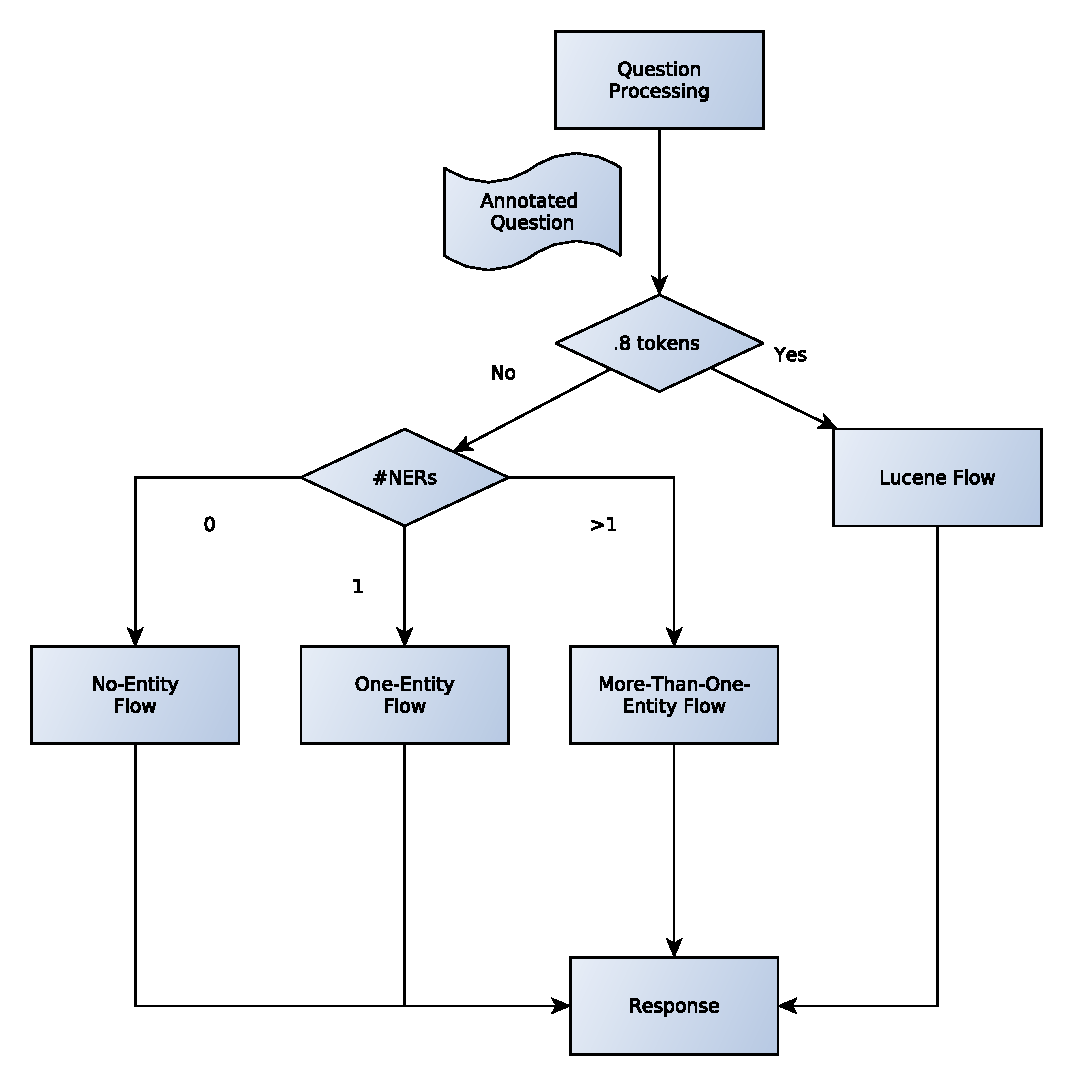
\includegraphics[scale=0.5]{graficos/AnswerRetrievalFlowEstructurado}
  \caption{Flow para la Generación de Respuestas - Estructurado}
  \label{fig:AnswerRetrievalFlowEstructurado}
\end{figure}

\subsubsection*{Ninguna o más de una entidad}
En el caso en el que no se haya identificado ninguna entidad del modelo quedan diferentes posibilidades, que se verifican en orden secuencial en base a nombres de colección, nombres de atributos, tipo de respuesta esperada y verbos. Los casos contemplados son: la pregunta por un campo de una colección (por ejemplo: direcciones de empresas en buenos aires) o por listas de entidades de una colección (investigadores de capital federal). Los diferentes casos son reglas de código escritas a mano. En todos los casos, si no se dan las condiciones para seguir especificando la dirección de la respuesta, se genera un respuesta ad-hoc con datos rankeados según el índice invertido, especificando de modo estructurado el camino recorrido hasta el momento. Por ejemplo, si se identifica que se pregunta por `investigadores' pero no es posible decidir ninguna especificación más (de capital federal, que hayan publicado en 2008, etc) entonces se retorna una lista de investigadores rankeada según el índice invertido `investigadores' con el resto de los datos de la pregunta. 

Por otro lado, si hay más de una entidad reconocida entonces hay sólo algunos casos posibles de relaciones entre ellas que pueden ser respuestas, que también se reflejan como caso de código. Finalmente, si no es posible identificar ninguno de estos caso, se toma un camino similar al mecanismo ad-hoc basado en information retrieval.


\subsubsection*{Una entidad}
El mejor caso es aquél en el que se reconocío una entidad y otros datos lingüisticos que permitan especificar qué se está preguntando. Al especificar acerca de qué/quién resulta mucho más sencillo canalizar qué se está preguntando. Los modelos que representan objetos (ver \allref{subsec:modelos-db}) son subclases de $NodoBase$, el cual representa una entidad en abstracto. Una entidad sabe responder preguntas acerca de ella. Para esto, utiliza las anotaciones de verbos, atributos nombrados y qwords para identificar qué se está preguntando. La pregunta puede responderse con un atributo o con una relación. Los distintos atributos de las distintas entidades se corresponden con verbos y con tipos de respuesta esperada. 

[[Detalle de casos y combinaciones de verbos + tipo de respuesta esperada + atributo]]
[[Ejemplos]]

\subsection{No Estructurado}

El proceso de generación de respuestas para los ejercicios de la Clef es muy distinto del anterior y puede dividirse en tres pasos principales: obtención de documentos y pasajes, ranking de pasajes y generación de respuesta. En el primer paso se accede a los índices invertido (al corpus) buscando documentos relevantes. Este paso pertenece netamente al área information retrieval. Como mencionamos al comentar Watson (en particular, ver \allref{subsec:deep-qa}), es fundamental que el resultado de este paso sea lo suficientemente amplio como para contener la respuesta pero lo suficientemente acotado como para no sobrecargar el proceso posterior de análisis lingüístico sobre los pasajes. Los documentos rankeados se dividen en pasajes. En el segundo paso, tanto los documentos como los pasajes son contrastados con distintas métricas contra los datos de la pregunta generando distintos valores para estos features. Finalmente, con esta información se procede al tercer paso, que consiste en realizar diferentes filtrados sobre los pasajes en función del tipo de respuesta esperado y en distintas formas de recopilar evidencia a favor de un pasaje o una entidad (depende el caso) para finalmente seleccionar una respuesta (o decidir que no se encontró ninguna).

\begin{figure}[H]
  \centering
    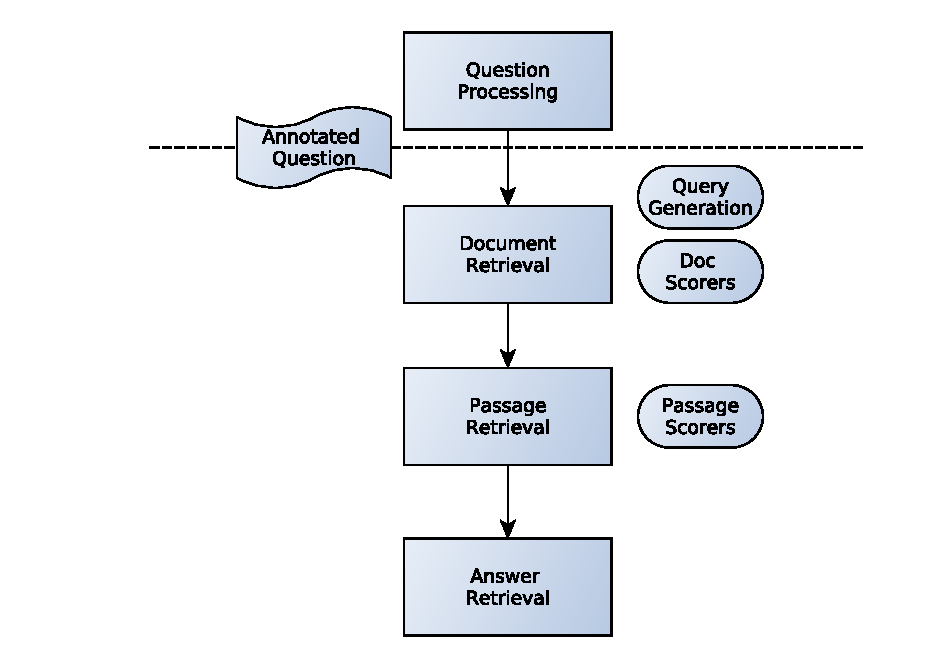
\includegraphics[scale=0.75]{graficos/AnswerRetrievalFlowWiki}
  \caption{Flow para la Generación de Respuestas - No Estructurado}
  \label{fig:AnswerRetrievalFlowWiki}
\end{figure}

\subsubsection{Documentos}
\label{subsec:docs}
En este punto, para una pregunta dada se dispone de la entidad del grupo de preguntas y de las distintas anotaciones hechas a la pregunta en el paso anterior (\allref{sec:qprocess}). Por su parte, los documentos en los índices invertidos poseen los campos $Id$, $Title$, y $Text$. El mecanismo de generación de queries tiene como objetivo priorizar en el ranking los documentos relacionados con el tema asociado al grupo de preguntas. Este paso es un problema de information retrieval puro: esto es, dado un pedido de información, retornar \textit{documentos relevantes}. El análisis semántico tiene peso en el paso posterior, a la hora de rankear pasajes. Por ejemplo, para el primer grupo de preguntas acerca de Harry Potter, solo se espera de este una lista de de documentos relacionados con ese mundo, en primer lugar. Por otro lado, es necesario que los principios de generación de queries no sean demasiado estrictos. Si en este punto quedan afuera muchas ocurrencias de una respuesta, entonces todo el resto del programa se ve afectado de manera irreparable. Es preferible generar documentos de más y luego filtrarlos mediante análisis lingüístico que ser demasiado estrictos y perder respuestas. 
Para lograr esto, ponderamos los documentos en los que las entidades nombradas reconocidas lingüísticamente aparecen en el título, si se dispone de más de una entidad buscamos documentos que mencionen ambos, luego priorizamos los documentos que poseen estas entidades dentro del cuerpo y también consideramos la presencia de verbos en diferentes conjugaciones y de sustantivos que ocurren en la pregunta. Finalmente, agregamos una lista de documentos enviando la pregunta misma como una query.  

Dado que finalmente se realizan queries simples (masivas), cabe preguntarse cual es la razón de la generación de queries y la ponderación de documentos. Esta razón es que en el proceso de ranking de pasajes y evaluación de respuesta se utilizan features basados en el score dado por lucene a los diferentes documentos. Si una mejor posición del documento contenedor del pasaje no implica que el pasaje sea correcto, si en cambio es un indicador de que dicho pasaje se encontró más cerca o más lejos del nucleo temático en el que se esperaba encontrarlo. 

Una vez generada la lista de documentos rankeados según lucene, se procede a analizar algunos features en base a distintos scorers propios. A su vez, estos distintos valores se combinan en una evaluación general del documento, que será utilizada luego a la hora de generar una respuesta. Estas dimensiones buscan en el título y en el artículo diferente medidas sobre las entidades nombradas y sobre la pregunta completa. En concreto, se miden distancias a la entidad nombrada que identifica al grupo de preguntas (ver \allref{subsec:entidad-de-grupo}), las entidades nombradad en la pregunta misma, a la pregunta completa y la respuesta esperada data. Las medidas contra la respuesta esperada -dada por Clef- no pueden usarse para generar la respuesta, pero sí para evaluar la performance del sistema. En el siguiente cuadro se muestran las dimensiones que se consideran sobre los documentos. 

\begin{center}
\begin{tabular}{| l | l | l |}
\hline
Entidad & Campo & Comparador \\ \hline
\multirow{6}{*}{Entidad de Grupo} & \multirow{3}{*}{Título} & Span \\ 
& & Covr \\
& & Freq \\ \cline{2-3}
& \multirow{3}{*}{Texto} & Span \\ 
& & Covr \\
& & Freq \\ \hline
\multirow{6}{*}{Entidades de Pregunta} & \multirow{3}{*}{Título} & Span \\ 
& & Covr \\
& & Freq \\ \cline{2-3}
& \multirow{3}{*}{Texto} & Span \\ 
& & Covr \\
& & Freq \\ \hline
\multirow{6}{*}{Todas las entidades} & \multirow{3}{*}{Título} & Span \\ 
& & Covr \\
& & Freq \\ \cline{2-3}
& \multirow{3}{*}{Texto} & Span \\ 
& & Covr \\
& & Freq \\ \hline
\multirow{6}{*}{Pregunta} & \multirow{3}{*}{Título} & Span \\ 
& & Covr \\
& & Freq \\ \cline{2-3}
& \multirow{3}{*}{Texto} & Span \\ 
& & Covr \\
& & Freq \\ \hline
\multirow{6}{*}{Respuesta} & \multirow{3}{*}{Título} & Span \\ 
& & Covr \\
& & Freq \\ \cline{2-3}
& \multirow{3}{*}{Texto} & Span \\ 
& & Covr \\
& & Freq \\ \hline
Score según índice & -- & -- \\ \hline
\end{tabular}
\end{center}

Los comparadores señalados ($Freq$, $Covr$, y $Span$) se utilizan en distintos lugares de esta tesis y su funcionamiento es explicado en el apéndice \allref{sec:comparadores}. Notar que `Entidades de la pregunta' refiere tanto a aquellas reconocidas por el NER-tagger como a construcciones sustantivadas y que `Pregunta' no es la pregunta bruta sino la priorización de verbos conjugados, sustantivos, adjetivos y entidades. 

El score general del documento es un cálculo ponderado de estas diferentes dimensiones. 

Lucene permite especificar cuántos documentos queremos recuperar. Para evaluar la performance de este paso, utilizamos medida distintos scores en base a la respuesta dada por dada por la conferencia para el ejercicio. Es importante notar que dado que no utilizamos las imagenes de wikipedia de la primera sugerencia, es esperable que las respuesta no estén `tal cual'. 
Evaluamos distintos mecanismos de generación de documentos, con distinta cantidad total, bajo distintas métricas. Para generar documentos, probamos la query trivial $ALL: pregunta$ (1), una un poco mejorada $ALL: entidad_de_grupo pregunta$ (2), secuencias concatenadas de queries tal como las describimos más arriba (3) y varios pedidos separados aplanados en un paso posterior (4). Para los cuatro métodos eliminamos los signos de puntuación. Para medir los resultados, utilizamos los comparadores de presencia exacta y diferentes grados de cobertura de términos (.8, .9 y 1). A su vez, evaluamos distintas imagenes de wikipedia para el español. Es total de preguntas del ejercicio, recordamos, es 200. Los resultados son los siguientes.

\begin{center}
\begin{tabular}{|l|l|l|l|l|l|l|}
\hline
Método & \# Docs & Wikipedia & Exacto & Covr 1 & Covr .9 & Covr . 8 \\ \hline

\multirow{6}{*}{1 - Trivial} & 
\multirow{3}{*}{100} & es - 2006 & 132 & 151 & 152 & 159 \\ 
 &  & es - 2007 & 144 & 159 & 160 & 164 \\
 &  & en - 2006 & x & x & x & x \\ \cline{2-7}
 & \multirow{3}{*}{1000} & es - 2006 & 144 & 167 & 167 & 173 \\ 
 &  & es - 2007 & x & x & x & x \\
 &  & en - 2006 & x & x & x & x \\ \hline

\multirow{6}{*}{2 - Trivial'} & 
\multirow{3}{*}{100} & es - 2006 & 138 & 156 & 157 & 164 \\ 
 &  & es - 2007 & 151 & 167 & 168 & 171 \\
 &  & en - 2006 & x & x & x & x \\ \cline{2-7}
 & \multirow{3}{*}{1000} & es - 2006 & 147 & 168 & 168 & 174 \\ 
 &  & es - 2007 & x & x & x & x \\
 &  & en - 2006 & x & x & x & x \\ \hline

\multirow{6}{*}{3 - Inteligente} & 
\multirow{3}{*}{100} & es - 2006 & 127 & 144 & 144 & 150 \\ 
 &  & es - 2007 & 141 & 150 & 151 & 156 \\
 &  & en - 2006 & x & x & x & x \\ \cline{2-7}
 & \multirow{3}{*}{1000} & es - 2006 & x & x & x & x \\ 
 &  & es - 2007 & x & x & x & x \\
 &  & en - 2006 & x & x & x & x \\ \hline

\multirow{6}{*}{4 - Inteligente'} & 
\multirow{3}{*}{100} & es - 2006 & 142 & 160 & 161 & 168 \\ 
 &  & es - 2007 & 157 & 170 & 171 & 174  \\
 &  & en - 2006 & x & x & x & x \\ \cline{2-7}
 & \multirow{3}{*}{1000} & es - 2006 & x & 147 & x & x \\ 
 &  & es - 2007 & x & 158 & x & x \\
 &  & en - 2006 & x & x & x & x \\ \hline
 
\end{tabular}
\end{center}

Conclusión de esto.

\subsubsection{Pasajes}
Este paso es análogo al anterior, pero con mayor detalle y granularidad. Cada documento generado en el paso anterior, con sus diferentes puntajes para 
las dimensiones señaladas, se parten en pasajes u oraciones. Nuevamente, sobre estas oraciones realizamos diferentes mediciones y las combinamos generando
un score final. En esta sección discutiremos las mediciones consideradas y los diferentes métodos de combinación de las mismas. Estos métodos de combinación generan distintos rankings de pasajes. Para evaluar estos rankings, nuevamente, utilizaremos la información disponible sobre las respuestas esperadas, buscando que la respuesta esperada se encuentre entre los $n$ pasajes mejor rankeados.
En primer lugar, las distintos scorers implementados son los siguientes:

\begin{center}
\begin{tabular}{| l | l | l |}
\hline
Comparador & Qué & Dónde \\ \hline
\multicolumn{3}{|c|}{Estadísticos} \\ \hline
Freq & Pregunta & Pasaje \\ \hline
Span & Pregunta & Pasaje \\ \hline
Covr & Pregunta & Pasaje \\ \hline
\#Tokens & -- & Pasaje \\ \hline
\multicolumn{3}{|c|}{Basados en NLP} \\ \hline
Presencia & Entidad de Grupo & Pasaje \\ \hline
Presencia & Entidades de pregunta & Pasaje \\ \hline
Presencia & Verbos de pregunta & Pasaje \\ \hline
Presencia & Sustantivos de pregunta & Pasaje \\ \hline
\multicolumn{3}{|c|}{Para evaluación} \\ \hline
Freq & Respuesta & Pasaje \\ \hline
Span & Respuesta & Pasaje \\ \hline
Covr & Respuesta & Pasaje \\ \hline
\end{tabular}
\end{center}

A estos Scorers se le suman los scores del documento asociado al pasaje (ver \allref{subsec:docs}). 
Sobre estas dimensiones disponibles, intentamos las siguientes combinaciones de priorización:

\begin{center}
\begin{tabular}{|l|l|l|}
\hline
\#& Nombre & Fórmula \\ \hline
1& Simple & $2+2=4$ \\ \hline
2& Respuesta & $2+2=4$ \\ \hline
3& Compleja & $2+2=4$ \\ \hline
\end{tabular}
\end{center}

Y consideramos la ocurrencia de respuestas, de la misma manera que en el apartado anterior (Match Exacto y tres medidas de covertura de tokens: 1, .9 y .8), 
sobre los primeros $n$ pasajes, con $n$ = 1, 5, 10, 20, 50 y 100.

\begin{center}
\begin{tabular}{|l|l|l|l|l|l|}
\hline
Fórmula & \#Docs & Exacto & Covr 1 & Covr .9 & Covr . 8 \\ \hline
\multirow{6}{*}{1} & 1 & x & x & x & x \\  \cline{2-6}
 & 5 & x & x & x & x \\ \cline{2-6}
 & 10 & x & x & x & x \\ \cline{2-6}
 & 20 & x & x & x & x \\ \cline{2-6}
 & 50 & x & x & x & x \\ \cline{2-6}
 & 100 & x & x & x & x \\ \hline
\end{tabular}
\end{center}


\subsubsection{Respuestas}





\begin{figure}
  \centering
    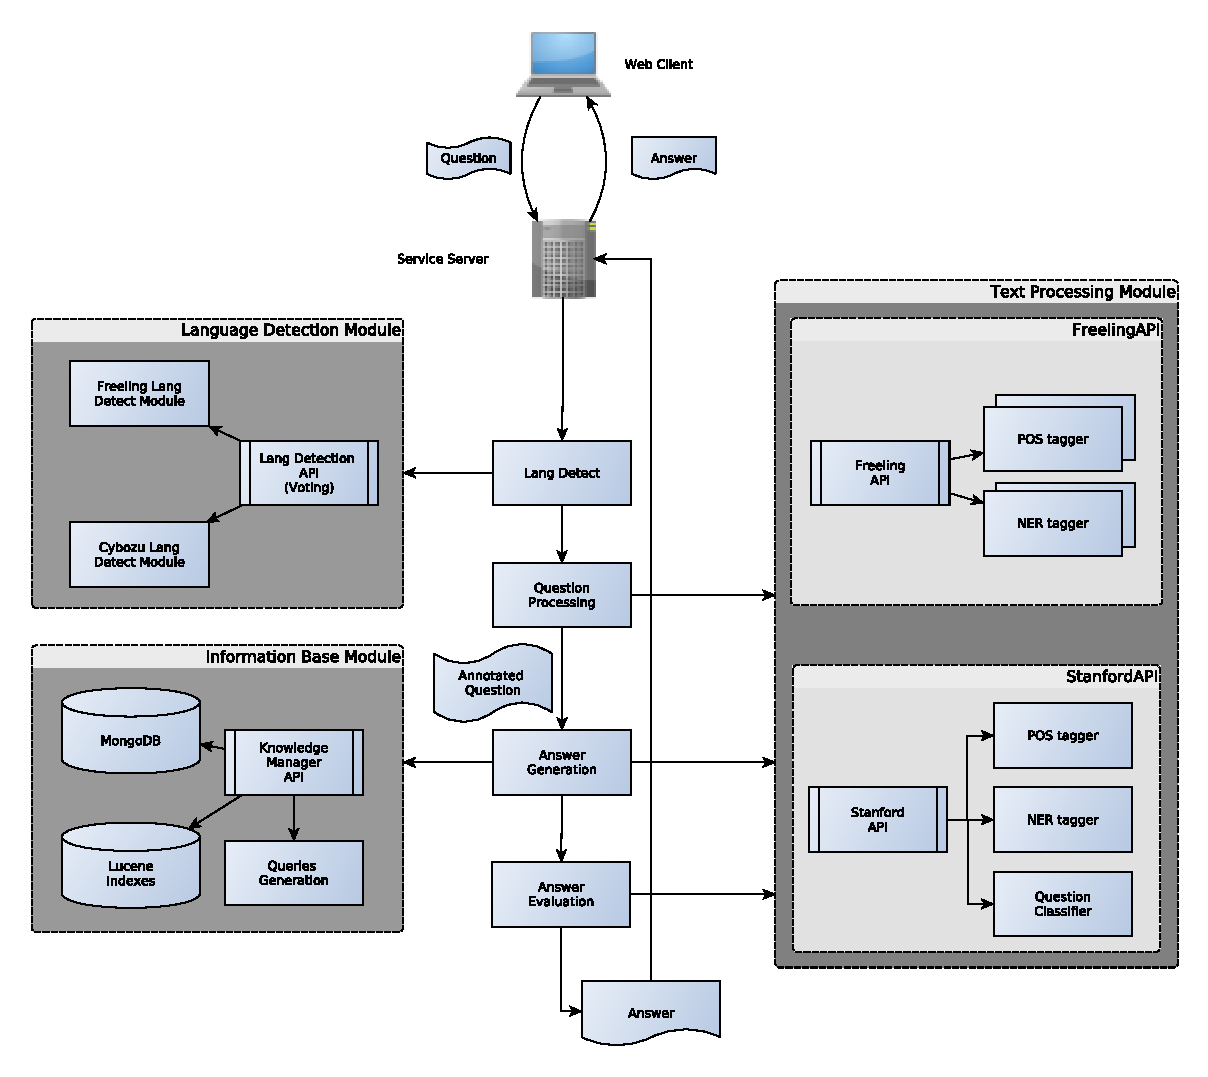
\includegraphics[scale=0.86]{graficos/Architecture}
  \caption{Arquitectura}
  \label{fig:Architecture}
\end{figure}

Como dice en \cite{greenwade93} y también en \cite{RE1}
%\end{document}


\section{Placeholders}

\subsection{Comentarios para estructurar 4}
Para multilingüe, creamos una api común con la api de freeling para stanford (aprovechar las ventajas de clasificador de stanford y adaptarlo al multilenguaje de freeling). 

\subsection{2 -Otras tecnologías}
Esta sección es un placeholder para las siguientes posibles tecnologías que podría describirse como última sección en \allref{chap:teorico}
\begin{itemize}
  \item Coreference Resolution \\
  Ejemplos de resolución de Freeling.
  \item Word sense disambiguation \\
  Hablar algo de wordnet?
  \item Relation Extraction \\
  La detección y extracción de relaciones es una tarea de procesamiento
de lenguaje natural que consiste en extraer entidades y relaciones semánticas
entre entidades a partir de un texto no estructurado. 

[[Escribir sobre distintos algoritmos conocidos basado en el paper RE1]]
  \item Machine Translation \\
    Hablar de los problemas con Google y otros y de las memorias de traducción. 
  \item Detección de idiomas \\
  La detección o identificación de idioma es la tarea de reconocer el
idioma de un cierto contenido. Esta tarea puede pensarse como una
tarea de clasificación donde las clases son los distintos
idiomas que el detector puede reconocer. 
  \item Shallow parsing (also chunking, "light parsing") \\
  is an analysis of a sentence which identifies the constituents (noun groups, verbs, verb groups, etc.), but does not specify their internal structure, nor their role in the main sentence.
It is a technique widely used in natural language processing. It is similar to the concept of lexical analysis for computer languages.
[[Expandir con detalles técnicos de wikipedia]]
\end{itemize}


\subsection{3- Conferencias y evaluaciones}
Conferencias
Precisión, recall y diferentes métricas para evaluar tomadas de distintos papers

\section{Secciones del apéndice}

\subsection{MyMemory}
MyMemory es la Memoria de Traducción más grande del mundo: 300 millones de segmentos a finales de 2009

Como las MT tradicionales, MyMemory almacena segmentos con sus traducciones, ofreciendo a los traductores correspondencias y concordancias. El proyecto se diferencia de las tecnologías tradicionales por sus ambiciosas dimensiones y por su arquitectura centralizada y basada en la colaboración colectiva. Todos pueden consultar MyMemory o hacer aportaciones a través de Internet; la calidad de las aportaciones será cuidadosamente ponderada.
MyMemory gives you quick access to a large number of translations originating from professional translators, LSPs, customers and multilingual web content. It uses a powerful matching algorithm to provide the best translations available for your source text. MyMemory currently contains 644.377.834 professionally translated segments.

Las memorias de traducción son almacenes compuestos de textos originales en una lengua alineados con su traducción en otras. Esta definición de memorias de traducción coincide literalmente con una de las definiciones más aceptadas de corpus lingüístico de tipo paralelo (Baker, 1995). Por esto se puede decir que las memorias de traducción son corpus paralelos.


Por el momento, no estamos utilizando ningún módulo de traducciones:
todo el enfoque multilingüe está dado por la detección del idioma
de la pregunta y la determinación de distintas herramientas de
análisis según qué idioma sea. Sin embargo, en un momento se
evaluó un enfoque distinto, basado en la traducción. Por ejemplo:
utilizar módulos de procesamiento sólo en inglés y
{\textquotedblleft}normalizar{\textquotedblright} los inputs en otros
idiomas (en principio, en espa\~nol), a este idioma interno, y luego lo
mismo con la generación de respuestas. A pesar de que no es el
enfoque actual, hubo una fase de investigación dentro del dominio de
la traducción, que resultó en un módulo de traducción basado en
MyMemoryAPI.

Intento con google translator y la privatización. ?`La falta de
software de traducción offline? El módulo de mymemory, robado de
algún lugar. El sistema de cobro. 

\subsection{Reverb}

ReVerb is a program that automatically identifies and extracts binary relationships from English sentences. ReVerb is designed for Web-scale information extraction, where the target relations cannot be specified in advance and speed is important.

ReVerb takes raw text as input, and outputs (argument1, relation phrase, argument2) triples. For example, given the sentence "Bananas are an excellent source of potassium," ReVerb will extract the triple (bananas, be source of, potassium).

\subsection{gwtwiki -Java Wikipedia API}\label{sec:gwtwiki}

Java Wikipedia API (Bliki engine)
http://code.google.com/p/gwtwiki/
Esta librería tiene métodos útiles para trabajar con dumps de wikipedia. La usamos para testear los métodos no estructurados de la tesis.


\subsection{Modelos de Morphia}\label{sec:modelos-morphia}

Java Wikipedia API (Bliki engine)
http://code.google.com/p/gwtwiki/
Esta librería tiene métodos útiles para trabajar con dumps de wikipedia. La usamos para testear los métodos no estructurados de la tesis.



\section{Conclusiones}
\section{Trabajo futuro}


\section{Citas a Textos trascriptos pero no usados}
\begin{itemize}
\item QC: \cite{QC1}, \cite{QC2} y también \cite{QC3} (y \cite{QC-other})
\item Clef: \cite{GuidelineClef07} y \cite{OverviewClef07} 
\item POS: El manual \cite{POS0} y los dos de Stanford: \cite{POS1} y \cite{POS2}
\item LangDetect: \cite{nakatani2010langdetect}
\item NER: Survey \cite{NER1} y el NER de Stanford: \cite{NER2}
\item Watson: \cite{WATSON1} y \cite{WATSON2}
\item Qanus: \cite{QANUS1}
\item RE: Survey \cite{RE1}, for QA \cite{RE2} y reverb: \cite{RE3}
\item Ephyra: \cite{EPHYRA1}
\item Freeling: \cite{FREELING1} y \cite{FREELING2} (este no impreso)
\item Wordnet para web ir: \cite{WN1} (no leido)
\item Varios de QA: Yago \cite{YAGO-QA1}, sobre una teoria de QA como interfaz a DBs: \cite{QADB1}. Corpus: \cite{TRAIN-QA1}, qall-me: \cite{QALL-ME1}, practical QA: \cite{QAS1}, simple QA: \cite{QAS2} y Surface de Ravishandran: \cite{SURF1}. Introducción a QA: \cite{QA1} y \cite{QA2} y \cite{QA3}
\item Aranea: \cite{ARANEA1} (no leido)
\item Passage retrieval evaluation: \cite{PASSAGE1}
\item Evaluacion de las TREC8 (metrica de \cite{QA3} LASSO): \cite{TREC8}
\item QA survey: \cite{QA-survey}
\end{itemize}

%% ...

% \appendix
%\nocite{*}

\begin{appendices}
  \appendix
\chapter{Herramientas}

\section{Stanford Question Classifier}
\label{sec:stanford-qc}
The question classifier (QuestionClassifier) is implemented with the 
STANFORD CLASSIFIER (Manning and Klein 2003), using the question taxonomy\footnote{http://cogcomp.cs.illinois.edu/Data/QA/QC/definition.html} 
explained in (Li and Roth 2002) and is responsible for finding out the expected 
answer type of a given question.

Li, Xin, and Dan Roth. "Learning Question Classifiers." International Conference 
on Computational Linguistics (COLING).2002.
Manning, Christopher, and Dan Klein. "Optimization, Maxent Models, and 
Conditional Estimation without Magic." Tutorial at HLT-NAACL and ACL. 2003.

This software is a Java implementation of a maximum entropy classifier.
Maximum entropy models are otherwise known as conditional loglinear
models, and are essentially equivalent to multiclass logistic
regression models (though parameterized slightly differently, in a way
that is advantageous with sparse explanatory feature vectors). 

\begin{center}
\begin{tabular}{| l | l |}
\hline
Clase y subclase & Definición \\ \hline
ABBREVIATION &  abbreviation \\ \hline 
  abb & abbreviation\\ \hline 
  exp & expression abbreviated\\ \hline 
ENTITY  & entities\\ \hline 
  animal  & animals\\ \hline 
  body & organs of body\\ \hline 
  color & colors\\ \hline 
  creative & inventions, books and other creative pieces\\ \hline 
  currency & currency names\\ \hline 
  dis.med. & diseases and medicine\\ \hline 
  event & events\\ \hline 
  food & food\\ \hline 
  instrument & musical instrument\\ \hline 
  lang & languages\\ \hline 
  letter & letters like a-z\\ \hline 
  other & other entities\\ \hline 
  plant & plants\\ \hline 
  product & products\\ \hline 
  religion  & religions\\ \hline 
  sport & sports\\ \hline 
  substance & elements and substances\\ \hline 
  symbol & symbols and signs\\ \hline 
  technique & techniques and methods\\ \hline 
  term  & equivalent terms\\ \hline 
  vehicle & vehicles\\ \hline 
  word & words with a special property\\ \hline 
DESCRIPTION & description and abstract concepts\\ \hline 
  definition & definition of sth.\\ \hline 
  description & description of sth.\\ \hline 
  manner & manner of an action\\ \hline 
  reason & reasons\\ \hline 
\end{tabular}
\begin{tabular}{| l | l |}
\hline
HUMAN & human beings\\ \hline 
  group & a group or organization of persons\\ \hline 
  ind & an individual\\ \hline 
  title & title of a person\\ \hline 
  description & description of a person\\ \hline 
LOCATION & locations\\ \hline 
  city & cities\\ \hline 
  country & countries\\ \hline 
  mountain & mountains\\ \hline 
  other & other locations\\ \hline 
  state & states\\ \hline 
NUMERIC & numeric values\\ \hline 
  code  & postcodes or other codes\\ \hline 
  count & number of sth.\\ \hline 
  date  & dates\\ \hline 
  distance &  linear measures\\ \hline 
  money & prices\\ \hline 
  order & ranks\\ \hline 
  other & other numbers\\ \hline 
  period  & the lasting time of sth.\\ \hline 
  percent & fractions\\ \hline 
  speed & speed\\ \hline 
  temp & temperature\\ \hline 
  size & size, area and volume\\ \hline 
  weight & weight\\ \hline 
\end{tabular}
\end{center}


\section{Stanford POS Tagger}

Part of Speech Tagging Stanford POS Tagger (Toutanova and Manning 
2000)

Toutanova, Kristina, and Christopher Manning. "Enriching the Knowledge 
Sources Used in a Maximum Entropy Part-of-Speech Tagger." Proceedings of 
the Joint SIGDAT Conference on Empirical Methods in Natural Language 
Processing and Very Large Corpora. 2000. 63-70.


\section{Stanford NER Tagger}
\label{sec:stanford-ner}

Named Entity Recognition Stanford Named Entity Recognizer (Finkel, 
Grenager and Manning 2005) 

Finkel, Jenny Rose, Trond Grenager, and Christopher Manning. "Incorporating 
Non-local Information into Information Extraction Systems by Gibbs Sampling." 
roceedings of the 43nd Annual Meeting of the Association for Computational 
Linguistics. 2005. \cite{NER2}


\section{Freeling}
\label{sec:freeling}
Freeling es una librería de c\'odigo abierto que provee distintas herramientas de 
procesamiento de lenguaje natural, desarrollada y mantenida por el Centre de Tecnologies 
i Aplicacions del Llenguatge i la Parla (TALP) de la Universidad Politécnica de Catalu\~na (UPC). 
Freeling está dise\~nado para ser usada como una librería externa y ofrece un API en distintos lenguajes
de programaci\'on. Su principal virtud es ser multilingüe, esto es, los diferentes analizadores que provee funcionan 
para un conjunto bastante amplio de idiomas. La última versi\'on a la fecha (3.1) soporta los siguientes idiomas:

\begin{itemize}
\item Asturian (as)
\item Catalan (ca) 
\item English (en)
\item French (fr) 
\item Galician (gl)
\item Italian (it)
\item Portuguese (pt)
\item Russian (ru)
\item Slovene (sl)
\item Spanish (es)
\item Welsh (cy)
\end{itemize}

Cabe destacar que no todos los m\'odulos soportan todos los idiomas. Sin embargo, dado que el proyecto está radicado en Espa\~na,
los idiomas necesarios para los fines de nuestro trabajo (espa\~nol e inglés), soportan todos los m\'odulos disponibles
en la librería.
Freeling 3.1 ofrece los siguientes analizadores lingüisticos:

\begin{itemize}
\item Detecci\'on de idioma
\item Tokenizer
\item Sentence splitting,
\item Análisis morfol\'ogico
\item NER y NEC (Detecci\'on y Clasificaci\'on de Entidades Nombradas)
\item Reconocimiento de fechas, números, magnitudes físicas, monedas
\item Codificaci\'on fonética
\item POS tagging, 
\item Shallow parsing
\item Dependency parsing
\item Wordnet-based sense annotation
\item Word Sense Disambiguation
\item Coreference resolution
\end{itemize}



\section{Lang Detect de Cybozu Labs}
\label{sec:cybozu}

Librería de Cybozu Labs - una compañía japonesa -, implementado en Java y liberado bajo Apache License 2.0. En la práctica, este paquete dio excelentes resultados. Soporta 53 idiomas con \%99 de precisión para todos ellos (según sus tests). El detector se basa en perfiles de idiomas generados a partir de las distintas wikipedias y detecta el idioma de los textos usando un filtro bayesiano ingenuo (\textit{naive bayesian}).
El código está disponible, actualmente, en google-code (El link está en la sección de bibliografía \cite{nakatani2010langdetect})

\section{MyMemory}
MyMemory es la Memoria de Traducción más grande del mundo: 300 millones de segmentos a finales de 2009

Como las MT tradicionales, MyMemory almacena segmentos con sus traducciones, ofreciendo a los traductores correspondencias y concordancias. El proyecto se diferencia de las tecnologías tradicionales por sus ambiciosas dimensiones y por su arquitectura centralizada y basada en la colaboración colectiva. Todos pueden consultar MyMemory o hacer aportaciones a través de Internet; la calidad de las aportaciones será cuidadosamente ponderada.
MyMemory gives you quick access to a large number of translations originating from professional translators, LSPs, customers and multilingual web content. It uses a powerful matching algorithm to provide the best translations available for your source text. MyMemory currently contains 644.377.834 professionally translated segments.

Las memorias de traducción son almacenes compuestos de textos originales en una lengua alineados con su traducción en otras. Esta definición de memorias de traducción coincide literalmente con una de las definiciones más aceptadas de corpus lingüístico de tipo paralelo (Baker, 1995). Por esto se puede decir que las memorias de traducción son corpus paralelos.


Por el momento, no estamos utilizando ningún módulo de traducciones:
todo el enfoque multilingüe está dado por la detección del idioma
de la pregunta y la determinación de distintas herramientas de
análisis según qué idioma sea. Sin embargo, en un momento se
evaluó un enfoque distinto, basado en la traducción. Por ejemplo:
utilizar módulos de procesamiento sólo en inglés y
{\textquotedblleft}normalizar{\textquotedblright} los inputs en otros
idiomas (en principio, en espa\~nol), a este idioma interno, y luego lo
mismo con la generación de respuestas. A pesar de que no es el
enfoque actual, hubo una fase de investigación dentro del dominio de
la traducción, que resultó en un módulo de traducción basado en
MyMemoryAPI.

Intento con google translator y la privatización. ?`La falta de
software de traducción offline? El módulo de mymemory, robado de
algún lugar. El sistema de cobro. 

\section{Reverb}

ReVerb is a program that automatically identifies and extracts binary relationships from English sentences. ReVerb is designed for Web-scale information extraction, where the target relations cannot be specified in advance and speed is important.

ReVerb takes raw text as input, and outputs (argument1, relation phrase, argument2) triples. For example, given the sentence "Bananas are an excellent source of potassium," ReVerb will extract the triple (bananas, be source of, potassium).

\section{Apache Lucene}
\label{sec:lucene}
Lucene es una librería de information retrieval, de c\'odigo abierto, escrita en Java y distribuida 
bajo la licencia Apache Software License por la Apache Software Foundation. No está pensada para
usuarios finales sino para ser integrada dentro de proyectos informáticos, resolviendo
la parte de bajo nivel y brindando servicios a través de un API en diferentes lenguajes de programaci\'on.
Su core es un índice invertido como el que describimos anteriormente. La implementaci\'on de un sistema
que utiliza Lucene consta de dos pasos separados:
\begin{itemize}
\item La \textbf{creaci\'on} del índice, es por lo general un proceso offline en el cual 
se incorporan distintas fuentes de informaci\'on al índice 
\item La \textbf{búsqueda} de documentos en el índice creado en el paso anterior, a partir de una query 
ingresada por el usuario final. Este proceso se incorpora dentro del flujo `online' del sistema.
El resultado de esta búsqueda es una lista de documentos rankeados con un cierto puntaje. 
\end{itemize}

Es importante señalar que si bien el proceso de creaci\'on del índice suele estar desacoplado del resto 
del sistema, las fuentes de informaci\'on no tiene por que ser `offline' en el sentido de ser documentos
en un disco local. De hecho, Nutch, otro proyecto de c\'odigo abierto de la Apache Software Foundation es 
un motor de búsqueda web basado en Lucene que incorpora un crawler para indexar sitios web. Lucene soporta 
cualquier fuente de informaci\'on que pueda convertirse en texto mediante algoritmia.
\newline
Los conceptos fundamentales de Lucene son: índice, documento, campo, término y query.
\begin{itemize}
\item Un índice contiene un conjunto de documentos
\item Un documento es un conjunto de campos
\item Un campo es el nombre de una secuencia de términos
\item Un término es un token (una palabra)
\item Una query es una lista de términos conectados con distintos operados l\'ogicos
\end{itemize}

\bigskip
[[Dar ejemplos de una query]]
\bigskip

\section{gwtwiki -Java Wikipedia API}\label{sec:gwtwiki}

Java Wikipedia API (Bliki engine)
http://code.google.com/p/gwtwiki/
Esta librería tiene métodos útiles para trabajar con dumps de wikipedia. La usamos para testear los métodos no estructurados de la tesis.


\section{Modelos de Morphia}\label{sec:modelos-morphia}

Java Wikipedia API (Bliki engine)
http://code.google.com/p/gwtwiki/
Esta librería tiene métodos útiles para trabajar con dumps de wikipedia. La usamos para testear los métodos no estructurados de la tesis.


\chapter{Comparadores}
\label{sec:comparadores}

Dada la frecuencia en la que resultaba necesario comparar dos string,
decidimos reificar la operación de comparación como una familia de
clases que implementan Comparadores. 


Gracias a esto se hace posible cambiar las nociones de igualdad o
similaridad en un módulo completo del sistema o en alguna clase
simplemente configurando otro comparador como parámetro. La
interfaz permite a los distintos comparadores tomar valores binarios
así como también valores entre 0 y 1. A su vez, esta considerada la
posibilidad de configurar un umbral (threshold) a partir del cual
redondear un valor entre 0 y 1 a un valor binario. Otro factor que tuvo
mucha utilidad fue la capacidad de anidar comparadores. 
El concepto de comparador incluye cualquier operación que tome dos
strings y genere un resultado booleano o analógico. Es decir, es posible 
incorporar análisis lingüísticos o queries a la base de datos en ellos.
También se incorpora la posibilidad de ignorar o no ignorar la diferencia de mayúsculas, 
y obviar o no las tildes y otros signos problemáticos. Los comparadores sirven,
en general, para comparar tanto strings representando palabras como
string representado listas de palabras (oraciones o textos). Algunos,
en particular, sólo sirven para este segundo caso. Los comparadores
que finalmente utilizamos en esta tesis son los siguientes.

\begin{center}
\begin{tabular}{| l | p {8cm} |}
\hline
\multicolumn{2}{|c|}{Comparadores de Strings} \\ \hline
Nombre & Descripción\\ \hline 
Equal & Compara por igualdad estricta \\ \hline 
EqualNoPunct &  Compara por igualdad, eliminando signos de
puntuación y normalizando acentos y otras posibles diferencias que no
deberían tenerse en cuenta. \\ \hline 
Contains & Verifica si un string contiene a otro. Puede usar Equal o EqualNoPunct \\ \hline 
EditDistance & Verifica cuan similares son dos string contando la mínima cantidad de operaciones requeridas para transformar un string en el otro \\ \hline 
\end{tabular}
\end{center}

Los siguiente comparadores son algoritmos fueron adaptados a partir de
los Scorers del proyecto Qanus. Todos devuelven valores reales entre
0 y 1 y sirven para comparar secuencias de tokens (y no sólo palabras). Estos
comparadores, al igual que Contains, no son simétricos. Para
distinguir, llamaremos primer string al buscado y segundo string a
aquel en el cual se busca el primero. 

\begin{center}
\begin{tabular}{| l | l | p {8cm} |}
\hline
\multicolumn{3}{|c|}{Comparadores de Secuencias de Tokens} \\ \hline
Abreviatura & Nombre &  Descripción\\ \hline 
Freq & Frequencia & Computa la cantidad de veces que los tokens del primer
string ocurren en el segundo string. Esta suma se divide por la
longitud del segundo string, dando un valor entre 0 y 1. \\ \hline 
Covr & Cobertura &  Computa cuantos tokens del primer string aparecen al
menos una vez en el segundo, y divide esta suma por el total de tokens
del \textit{primer} string.\\ \hline 
Prox & Proximidad &  Computa la distancia entre dos strings en un tercero. Ver abajo.   \\ \hline 
Span & Distancia entre tokens & Computa la distancia media entre términos del primer string en el segundo. Ver abajo. \\ \hline
\end{tabular}
\end{center}

Vamos a explicar los algoritmos de $Prox$ y $Span$ ya que no son triviales. \newline
$Prox$ toma dos strings a buscar en un tercero. Busca ambos en el tercero y computa la distancia en tokens entre ellos.
Esta distancia se calcula como la distancia entre el centro de ambos strings.
Por ejemplo, para los strings de búsqueda \dq{Argentina es un país americano} y \dq{independizado en 1810} sobre el texto \dq{Argentina es un país americano, originalmente una colonia española, independizado en 1810} se considera la distancia entre \sq{un} y \sq{en} (por ser los tokens \sq{intermedios} de ambos strings
de búsqueda. La distancia entre ambos, en el tercer string, es 7. Esta distancia se divide por la longitud en tokens del string en el que se buscan (12), dando un resultado de 0.58. Un score cercano a 1 denota que los dos string están cercanos uno al otro en el tercer string. \newline
Por su parte, $Span$ tiene un concepto similar, pero funciona sobre un solo string de búsqueda, considerando sus tokens. Los distintos tokens buscados ocurren en ciertas posiciones. $Span$ considera la distancia entre las posiciones de los tokens más distantes, dividiendo el total de tokens encontrados por este valor.
Un score cercano a 1 significa que los términos del string buscado están cerca en el string en el que se buscan.
Por ejemplo, suponiendo los siguientes matchs de tokens (denotados por una X): \newline
..... X ..... X ..... X ...... \newline
......a ...... b ...... c ...... \newline

El score de $Span$ estaría dado por \#total de tokens encontrados /  {\textbar}c-a{\textbar}.

\end{appendices}

%%%% BIBLIOGRAFIA
\backmatter
\bibliographystyle{apalike}
\cleardoublepage
\phantomsection
\addcontentsline{toc}{chapter}{Bibliografía}
\bibliography{tesis}


\end{document}
